\documentclass[a4paper,11pt,openright,oneside]{book}
\frenchspacing

\usepackage[utf8]{inputenc}
\usepackage[italian]{babel}
\usepackage[dvips]{graphicx}
\usepackage{url}
\usepackage{rotating}
\usepackage{verbatim}
\usepackage{longtable}
\usepackage[boxed]{algorithm2e}
\usepackage{amsmath}

\usepackage{amssymb} %simboli matematici
\usepackage{latexsym} %?
\usepackage{mathrsfs} %?
\usepackage{amsfonts}

\usepackage{multirow}

\usepackage{hyperref}

\usepackage{frontespizio}
\usepackage{listings} %Per inserire codice
\usepackage[usenames]{color}%Per permettere la colorazione dei caratteri 
\usepackage{fancyhdr} 


\usepackage{listings} %Per inserire codice
\usepackage[usenames]{color}%Per permettere la colorazione dei caratteri 

\usepackage{titlesec,blindtext}
\usepackage[Lenny]{fncychap}

\usepackage{eso-pic}
\newcommand\BackgroundPicture{
   \put(0,0){
     \parbox[b][\paperheight]{\paperwidth}{
       \vfill
       \centering
       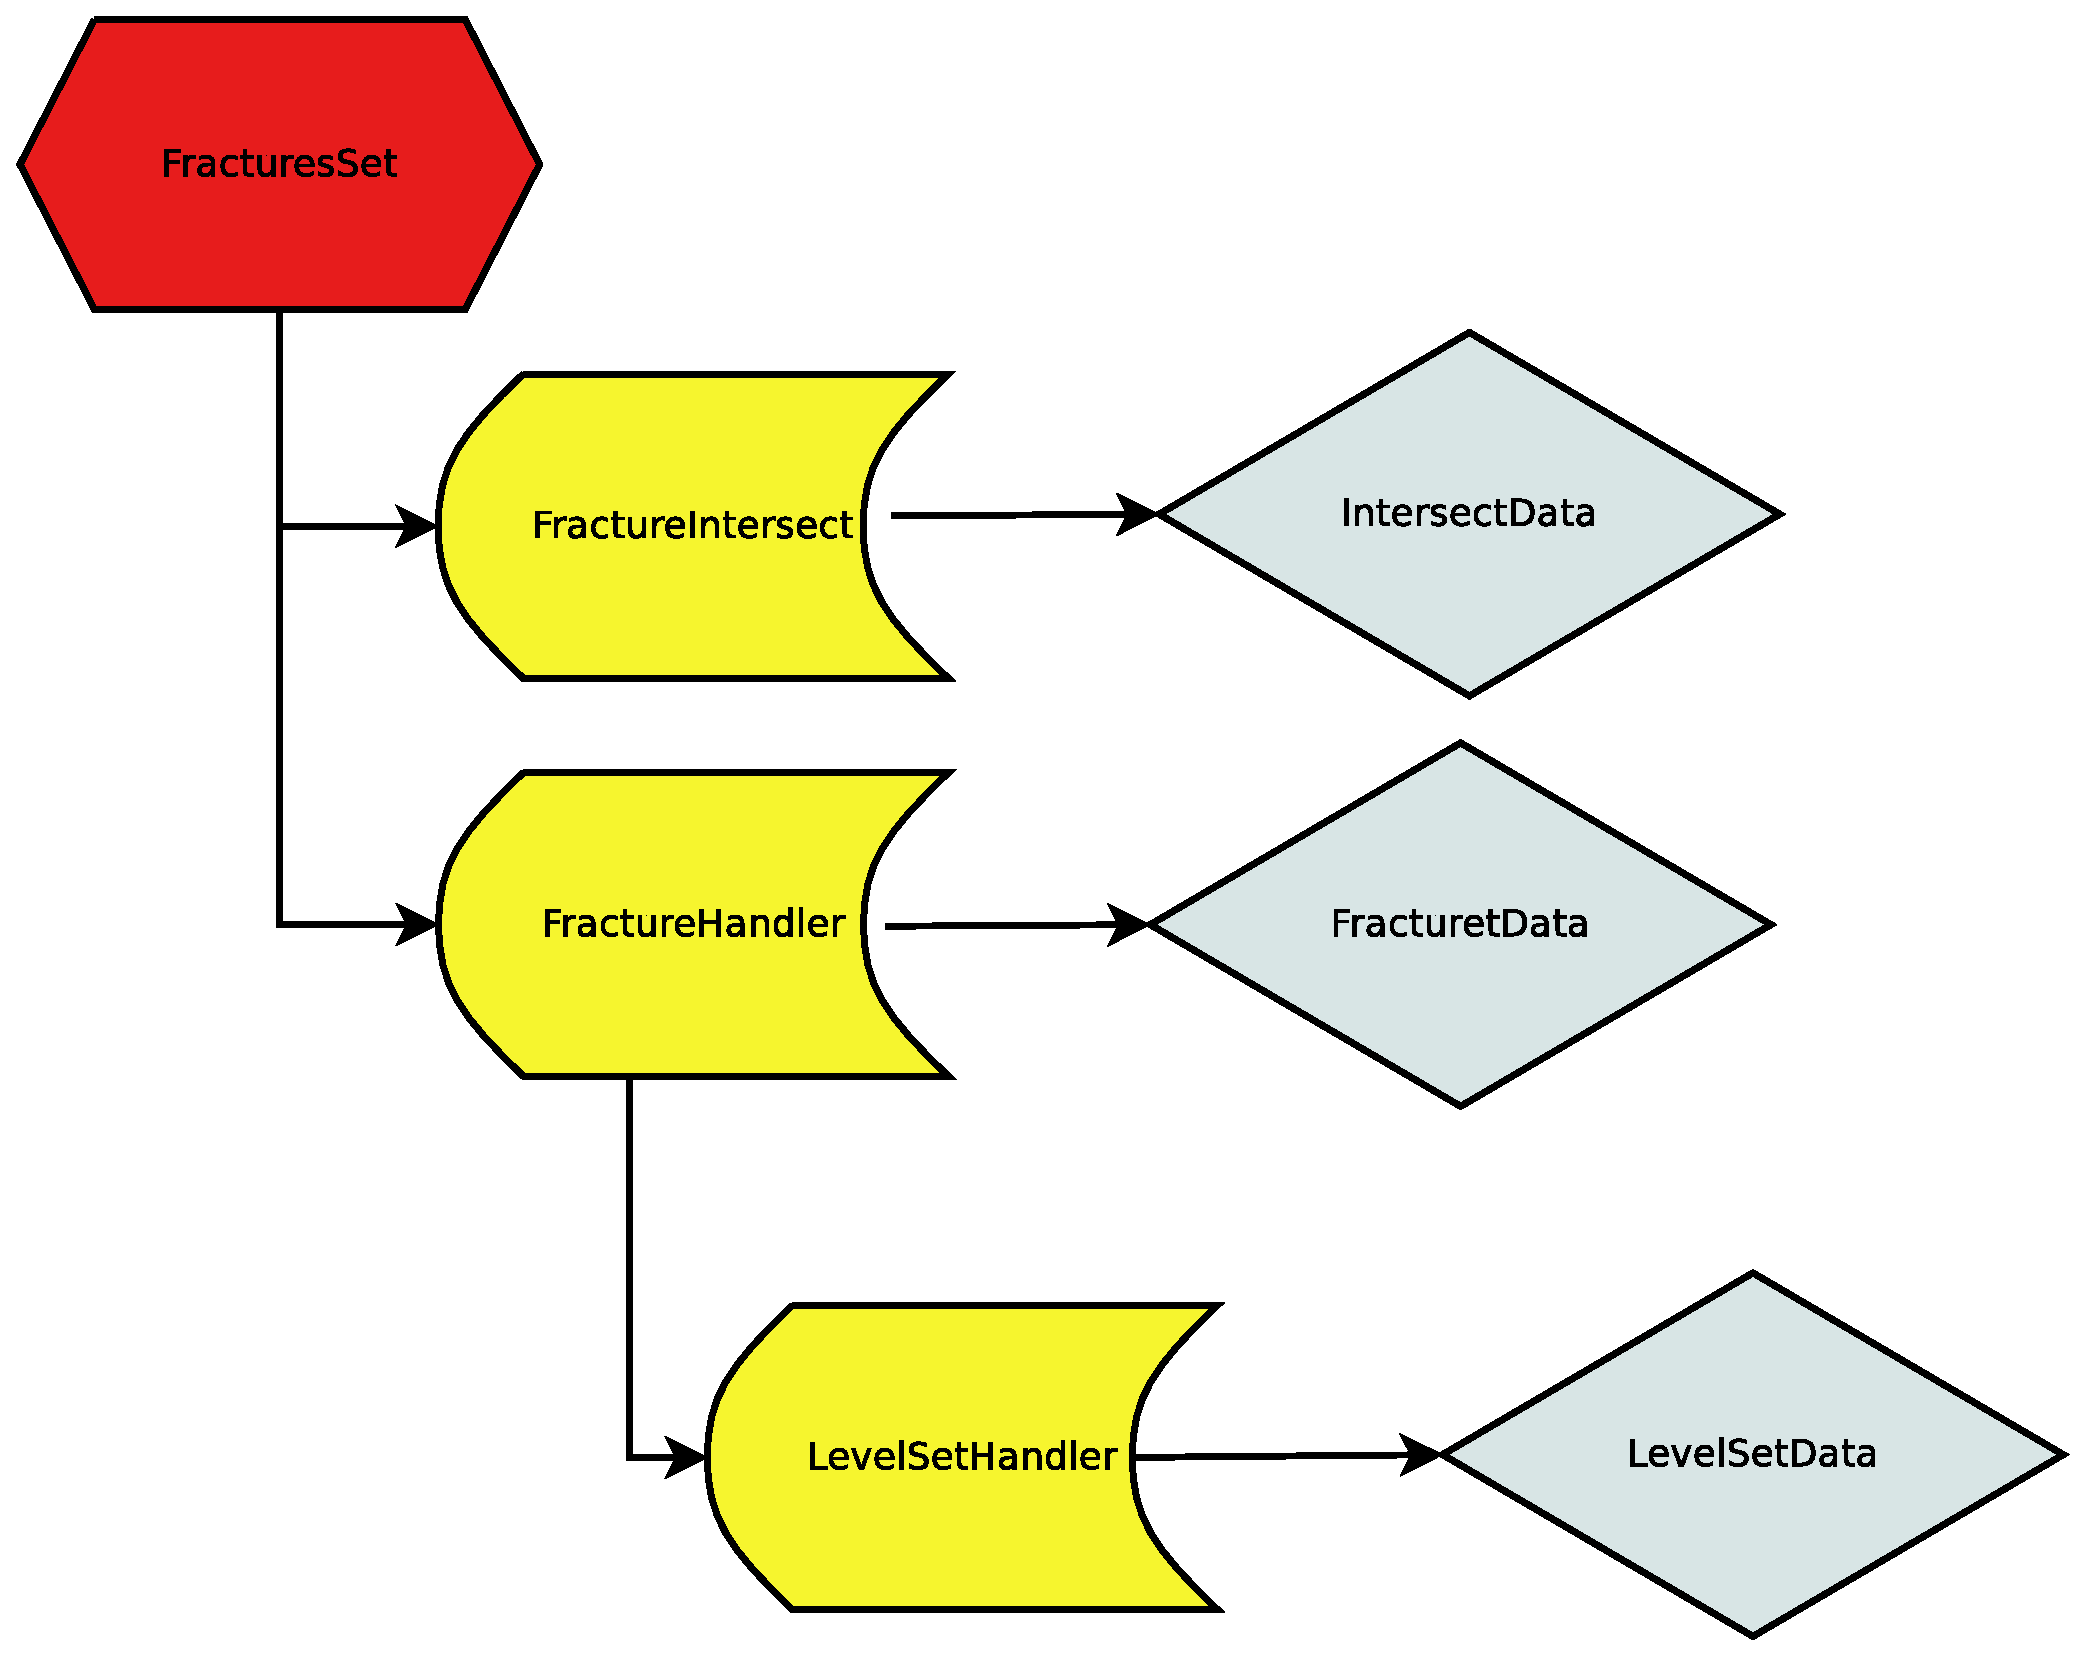
\includegraphics[width=\textwidth]{img/fratture.eps}
       \vfill
     }}}



%\usepackage[Sonny]{fncychap}
%\usepackage[toc]{glossaries}
%\makeglossaries
%\usepackage{lscape}

\ChNameVar{\fontsize{14}{16}\usefont{T1}{phv}{m}{n}\selectfont}
\ChNumVar{\fontsize{60}{62}\usefont{T1}{ptm}{m}{n}\selectfont}

 
\begin{document}

\begin{frontespizio}

\Istituzione{POLITECNICO DI MILANO}
\Logo{logo_polimi}
\Facolta{Ingegneria Industriale e dell'informazione}
\Corso[Laurea]{Ingegneria Matematica}
\Annoaccademico{2013-2014}
\Sottotitolo{Imposizione delle condizioni d'interfaccia per intersezioni di tipo Biforcazione}
\Titolo{\color[rgb]{.6,0,0} Soluzione del problema di Darcy in un network di fratture}
\Candidato[]{Claudia Bonomi matr. 804378}
\Candidato[]{Maria Iemoli matr. 800499}
\Titoletto{Progetto per il corso di Programmazione Avanzata per il Calcolo Scientifico}
\Relatore{ Luca Formaggia}
\Relatore{ Anna Scotti}
\Rientro{1cm}
\Margini{1.5cm}{2cm}{1.5cm}{3cm}
\end{frontespizio} 


\hypersetup{
    %colorlinks,
    citecolor=black,
    filecolor=black,
    linkcolor=black,
    urlcolor=black
}


%\maketitle

%\hyphenation{net-list}\pagestyle{empty}
%
\usepackage[latin1]{inputenc}
\usepackage[italian]{babel}
\usepackage{latexsym}
\usepackage{epsfig}
\usepackage{tabularx}
\usepackage{morefloats}
\usepackage{setspace} 
\usepackage{url}
\usepackage[sans,nouppercase]{frontespizio}



%\begin{document}
\begin{frontespizio}
\Universita{Politecnico di Milano}
\Logo{logo_polimi}
\Facolta{Scuola di Ingegneria Industriale e dell'Informazione}
\Corso{Ingegneria Matematica}
\Annoaccademico{2013--2014}
\Titoletto{Progetto per il corso di ANEDPII}
\Titolo{Segmentazione del Ventricolo Sinistro con tecniche GAC}
\Candidato[800499]{Maria Iemoli}
\Relatore{Simona Perotto}
\Relatore{Elena Faggiano}
\end{frontespizio}



%\newpage
\chapter*{Introduzione}

Il presente progetto si inserisce nell'ambito dello studio del moto di un fluido in un mezzo poroso.\cite{habilitationsschrift}
Lo scopo è quello di studiare e risolvere il problema nel caso di un network di fratture che si intersecano. \\
Il nostro progetto parte da un codice già esistente in C++ in grado di risolvere il problema di Darcy nel caso in cui due fratture abbiano un'intersezione a \textit{X}. \cite{ESAIM}
Il nostro obiettivo è quello di estendere il codice ad altri tipi di intersezione, in particolare vogliamo risolvere il problema in presenza di tre fratture che si intersecano in un unico punto comune formando una \textit{Y}.\\
Per l'implementazione e la risoluzione del problema tramite elementi finiti, abbiamo utilizzato principalmente la libreria \texttt{GetFEM++}, un insieme di liberie scritte in C++ che mettono a disposizione dell'utente una serie di funzioni utilizzabili per la soluzione dei problemi FEM. \\
La nostra implementazione si basa su un modello ridotto, considera cioè le fratture come delle grandezze 1d, trascurandone lo spessore. Per poter ricavare le condizioni d'interfaccia nel caso della nuova intersezione si è reso necessario ritornare al modello 2d, e quindi considerare l'intersezione come un triangolo e non come un punto \cite{Paper} \cite{LDAP}.

\pagestyle{plain}
\pagenumbering{Roman}
\include{prefazione}

\pagenumbering{arabic}
\tableofcontents

\chapter{Mezzi porosi e legge di Darcy}

I materiali porosi sono dei mezzi in cui si possono distinguere due costituenti: una matrice solida, la parte che costituisce la struttura rigida del corpo, e lo spazio vuoto restante, che può essere riempito con uno o più fluidi. \\
Risulta spesso interessante studiare il moto di un fluido in un mezzo poroso in cui sia possibile distinguere delle fratture o dei canali al suo interno. Nell'analisi del moto di un fluido in una frattura tra diversi strati geologici, ad esempio,  si può pensare che il fluido, oltre a insinuarsi e scorrere nella frattura, si propaghi mediante filtrazione negli strati adiacenti la frattura stessa.
Un'altra possibile applicazione in ambito idrogeologico riguarda lo studio di come i fiumi irrighino il terreno ad essi circostante. 
\par Il moto del fluido all'interno del mezzo poroso viene descritto tramite la legge di Darcy.  Generalmente le dimensioni delle fratture sono di molto inferiori a quelle del dominio occupato dal mezzo poroso. Questo ha portato allo sviluppo di tecniche per lo studio del flusso all'interno delle fratture basate su modelli ridotti. Questi modelli si inseriscono nella categoria dei modelli multiscala, ed hanno il vantaggio di evitare la risoluzione del campo di moto sulle scale spaziali molto piccole nella frattura.

\section{Legge di Darcy}
La legge di Darcy descrive la filtrazione di un fluido incomprimibile all'interno di un mezzo poroso. In particolare costituisce un legame tra il campo di velocità del fluido e il gradiente di pressione nel mezzo poroso. \\
Il moto di un fluido incomprimibile in un mezzo poroso ( considerando z=0 come quota di riferimento) può essere descritto dalla seguente coppia di equazioni:
 
\begin{equation}
\textbf{u} =- \frac{\textbf{K}}{\mu}\nabla {p} \footnote{Più avanti indicheremo $\frac{\textbf{K}}{\mu}$ con $\textbf{K}$ per semplicità}
\end{equation}\label{Darcy}

\begin{equation}
\nabla \cdot u =f
\end{equation}

dove:
\begin{enumerate}
\item[-] \textbf{u}(\textbf{x}, t) è il campo di velocità macroscopica del fluido misurata in [\textit{m/s}];
\item[-] \textbf{K}(\textbf{x}) è il tensore simmetrico di permeabilità assoluta misurato in [\textit{m$^2$}];
\item[-] \textit{p}(\textit{x,t}) è la pressione del fluido in [\textit{Pa}]=[\textit{N/m$^2$}];
\item[-] \textit{$\mu$} (\textbf{x}, t) rappresenta la viscosità dinamica del fluido in [\textit{Pa s}], che per semplicità verrà considerata costante;
\item[-] \textit{f}(\textbf{x}, t) rappresenta il termine sorgente di dimensione [\textit{s}$^{-1}$].
\end{enumerate}


La prima equazione è la legge di Darcy e deriva dalla conservazione del momento nelle equazioni di Navier-Stokes con opportuni passaggi, mentre la seconda rappresenta la conservazione della massa. \\
L'approssimazione con il modello di Darcy è valida per fluidi Newtoniani con bassi valori del numero di \textit{Raynolds} ($Re<10$), per cui gli effetti inerziali possono essere trascurati. Per valori maggiori è necessario estendere il modello poichè l'equazione \ref{Darcy} presenta dei limiti.


 \section{Formulazione debole del problema}
Il problema del flusso di un fluido in un mezzo poroso assume la seguente forma:

\begin{equation}
\begin{cases}
\textbf{K}^{-1}  \textbf{u} +\nabla {p} =0 \\
\nabla  \cdot u =f
\end{cases} 
\end{equation}\label{sistema}

\noindent con condizioni al contorno:

\begin{equation}
\begin{cases}
\textbf{u} \cdot \textbf{n}_{\Omega} =0  & su \;  \Gamma ^u\\
p =g & su \; \Gamma ^p
\end{cases}
\end{equation}\label{bc}

Per ricavare la formulazione debole del problema, così da poter discretizzare con gli elementi finiti, moltiplichiamo la prima equazione del sistema \ref{sistema} per una funzione test \textbf{v}, la seconda per una funzione test \textit{q} e integriamo su $\Omega$. \\
La formulazione debole diventa: trovare (\textbf{u}, $p$) tali che:
\begin{equation}
\begin{split}
\int_{\Omega} (\textbf{K}^{-1} \textbf{u}) \cdot \textbf{v} \, dx  - \int_{\Omega} p \nabla \cdot \textbf{v} \, dx  + \int_{\Gamma^p} g \, \textbf{u} \cdot \textbf{n} \, d\Gamma = 0 & \quad  \forall \, \textbf{v} \in \textbf{W} \\
\int_{\Omega} \nabla \cdot \textbf{u} q \, dx = \int_{\Omega} f q \, dx & \quad \forall \, q \in Q
\end{split}
\end{equation}\label{formdebole}

dove: 

\begin{equation*}
\begin{split}
\textbf{W} &=H_{div}(\Omega) = \left \{ \textbf{w}\in [L^2(\Omega)]^2, \nabla \cdot \textbf{w} \in L^2(\Omega), \textbf{v} \cdot \textbf{n} = 0 \, su \, \Gamma^n \right \} \\
Q &= L^2(\Omega) 
\end{split}
\end{equation*}

Per la discretizzazione in spazio scegliamo lo spazio degli elementi finiti di grado due per la velocità e uno per la pressione e ricaviamo la seguente formulazione algebrica:
\begin{equation}
\begin{cases}
A_{11} \textbf{U} \, +A_{12} \textbf{P} = F_1 \\
A_{12}^T \textbf{U} = F_2
\end{cases}
\end{equation}


dove $ A_{11} \in \mathbb{R}^{N_u \times N_u}$ e $A_{12} \in \mathbb{R}^{N_p}$  sono le matrici realative alle forme bilineari $a(\cdot, \cdot)$ e $b(\cdot, \cdot)$ definite come:

$$ a(\textbf{u}_h , \textbf{v}_h)= \int_{\Omega} (\textbf{K}^{-1} \textbf{u}_h) \cdot \textbf{v}_h \, dx \qquad b(\textbf{u}_h, q) = - \int_{\Omega} q_h \nabla \cdot \textbf{u}_h \, dx  $$
$$ f1(\textbf{u}_h) = \int_{\Gamma^p} g_h \, \textbf{u}_h \cdot \textbf{n} \, d\Gamma \qquad f2(q_h) =  - \int_{\Omega} f q \, dx $$

Nel nostro caso quindi, per risolvere il flusso di un fluido all'interno di una frattura in un mezzo poroso si ottiene il seguente sistema algebrico:
\begin{equation}
\left[\begin{matrix}A_{11} &A_{12} \\A_{12}^T & 0 \end{matrix}\right] \, \left[\begin{matrix}U  \\P \end{matrix}\right] = \left[\begin{matrix}F_{1} \\F_{2} \end{matrix}\right] 
\end{equation}
\label{sistemaAlgebrico}

Se vi sono più fratture che si intersecano è necessario imporre delle condizioni che leghino i rispettivi flussi e le rispettive pressioni. Il codice da cui siamo partite impone le condizioni d'interfaccia nel caso di un'intersezione di tipo \textit{Cross} in modo debole. Il nostro codice, come verrà spiegato più avanti, impone le condizioni d'interfaccia nel caso della \textit{Biforcazione} in maniera forte, ossia una volta che il sistema algebrico è già stato assemblato.
\lstnewenvironment{Code03_01}[1][]{ \lstset{showspaces=false, showtabs=false,tabsize=2,basicstyle=\small\ttfamily, columns=fullflexible,framexrightmargin=+.1\textwidth, keywordstyle=\color{red}\bfseries, commentstyle=\color{blue},language=C++, basicstyle=\small,  numberstyle=\tiny, stepnumber=1, numbersep=5pt, frame=shadowbox, #1}}{}


\chapter{Considerazioni preliminari}

\section{Strumenti di sviluppo}
Lo sviluppo del nostro progetto ha richiesto l'uso di strumenti specifici atti a facilitare e sistematizzare la gestione del codice quali \texttt{git}, \texttt{CMake} e \texttt{Doxygen}.\\

\subsection{\texttt{Git}}
\href{https://github.com/}{\texttt{Git}} è un sistema di controllo versione utilizzabile direttamente da linea di comando, molto diffuso è utile per tenere traccia delle varie fasi di sviluppo del codice. Git gestisce in modo adeguato i contributi al codice provenienti da agenti esterni e permette la condivisione del codice.\\
Il codice del progetto è reperibile su \texttt{git} ed è possibile scaricarlo e collabolare allo sviluppo clonando il codice dalla repository  \href{https://github.com/}{\texttt{GitHub}}:\\
\begin{center}
\texttt{ git clone https://github.com/mariaiemoli/progetto.git}
\end{center}
Nella cartella principale è contenuto anche un file \texttt{.gitignore}, in cui sono specificate le estensioni dei files e le sottocartelle che non devono essere visionati in una repository \texttt{git}. In particolare non si è interessati ai files temporanei che vengono eventualmente generati dagli editor, e alle cartelle generate da uno scorretta configurazione di \texttt{Doxygen}.

\subsection{\texttt{CMake}}
\href{http://www.cmake.org/}{\texttt{CMake}} è un software libero multipiattaforma nato per l'automazione dello sviluppo. Sostanzialmente con l'uso di \texttt{CMake} è possibile configurare e generare Makefile per il sistema operativo in uso. Questo facilita la diffusione del codice tra sviluppatori, non dovendo far altro che lanciare \texttt{CMake} e lasciare che sia lui ad occuparsi della ricerca di compilatori e librerie locali e della costruzione di software.\\
\texttt{CMake} si basa sulla creazione di files \texttt{CMakeLists.txt} nella directory del progetto, che contengono le direttive necessarie per creare il \texttt{Makefile} per compilare ed eseguire il codice. \\
Nella directory principale si trova un primo file \texttt{CMakeLists.txt} in cui si impostano i parametri fondamentali quali la dipendenza dalla versione di \texttt{CMake}, il nome del progetto, si includono le directory dei sorgenti nel path di compilazione e si caricano le librerie esterne utilizzate dai sorgenti. \\
Le librerie che vengono caricate sono:
\begin{enumerate}
\item[-] \texttt{Eigen}, libreria template per l'algebra lineare usata principalmente nella fase di imposizione delle condizioni di interfaccia sul triangolo di intersezione nel caso della biforcazione, per il modello ridotto;
\item[-] \texttt{Getfem++}, libreria matematica per gli elementi finiti usata per scrivere e risolvere il problema numerico;
\item[-] \texttt{Blas} (Basic Linear Algebra Subprograms) e \texttt{Qhull}, librerie necessarie per \texttt{Getfem++};
\item[-] \texttt{Doxygen}, usato per generare la documentazione
\end{enumerate}

\begin{Code03_01}
CMAKE_MINIMUM_REQUIRED( VERSION 2.8 )

PROJECT(PACS)

SET(CMAKE_CXX_FLAGS "-std=c++0x -Wall ${CMAKE_CXX_FLAGS}")

SET(CMAKE_MODULE_PATH 
	${CMAKE_SOURCE_DIR}/cmake ${CMAKE_MODULE_PATH})

# Include Eigen3
FIND_PACKAGE(PkgConfig)
PKG_CHECK_MODULES(EIGEN3 REQUIRED eigen3)
INCLUDE_DIRECTORIES(${EIGEN3_INCLUDE_DIRS})

# Include Doxygen
find_package(Doxygen)
[ ... ]

# Include Getfem
if (GETFEM_LIBRARIES AND GETFEM_INCLUDE_DIRS)
[ ... ]

#Include for BLAS library
find_package ( BLAS )
[ ... ]


#Include for LAPACK library
find_package ( LAPACK )
[ ... ]

#Include for QHULL library
set(QHULL_MAJOR_VERSION 6)
[ ... ]

SET(CMAKE_INSTALL_PREFIX 
${CMAKE_SOURCE_DIR}/install-dir CACHE PATH "" FORCE)

ADD_SUBDIRECTORY(src)
ADD_SUBDIRECTORY(test)
\end{Code03_01}

%% $

Per poter usare \texttt{CMake} è necessario posizionarsi nella directory in cui è contenuto il progetto e creare una cartella in cui compilare il codice. Per lanciare \texttt{CMake} è necessario digitare i seguenti comandi: \\ 

\par  \texttt{cd $<$build\_dir$>$ } 
\par \texttt{cmake $<$source\_dir$>$}\\

\noindent \texttt{CMake} imposta le variabili di path come definito nel file  \texttt{CMakeLists.txt}, esamina le dipendenze da librerie esterne e procede esaminando le sottocartelle aggiunte nel file di configurazione. In particolare esamina le sottocartelle \texttt{src} e \texttt{test}, in cui sono presenti altri files  \texttt{CMakeLists.txt}, che impostano i rispettivi obiettivi e definiscono le rispettive sottocartelle. Questo permette a \texttt{CMake} di esaminare tutta la directory in cui è contenuto il progetto in maniera ricorsiva. \\
%Nella cartella \texttt{src} il file  \texttt{CMakeLists.txt} aggiunge la creazione di una libreria a partire dal codice del progetto. \\
%\begin{Code03_01}
%ADD_LIBRARY(pacs ${TARGET_SRC} ${TARGET_HANDLER})
%\end{Code03_01}

\par \noindent Nella cartella test si trovano delle sottocartelle contenenti un file data di esempio per poter eseguire il codice e un file  \texttt{CMakeLists.txt} .\\
\noindent Il file  \texttt{CMakeLists.txt} nella cartella dei test definisce gli obiettivi e i collegamenti necessari per l'esecuzione. \\

\noindent Una volta che il \texttt{Makefile} è stato generato è possibile compilare il codice con il comando: \\ 
\par \texttt{make}\\

\noindent Questo crea in ogni sottocartella della cartella \texttt{test} un eseguibile chiamato \texttt{Test}. Per poterlo eseguire è sufficiente lanciare da terminale, dopo essersi posizionati nella directory corretta, 
\par \texttt{ .\textbackslash Test-iesimo }

\subsection{\texttt{Doxygen}}
\href{www.doxygen.org/}{\texttt{Doxygen}} è un sistema multipiattaforma molto diffuso per la generazione automatica della documentazione di un codice. Per ottenere la documentazione è necessario introdurre nel codice dei commenti con una sintassi particolare, e il risultato contiene l’elenco delle classi implementate, i loro diagrammi di collaborazione e la descrizione di metodi ed attributi.
Per poter creare la documentazione al codice con \texttt{Doxygen} è necessario che nella cartella principale sia presente il file \texttt{Doxygen}, in caso contrario è necessario crearlo con il comando:\\
\par \texttt{Doxygen -g}\\

\noindent In questo file sono definite le variabili che permettono di creare la documentazione come il nome del progetto, la directory dove creare la documentazione, le cartelle dove si trovano i sorgenti e l'estensione dei files da considerare.

\begin{Code03_01}
PROJECT_NAME 				=	 Problema di Darcy in un network di fratture
OUTPUT_DIRECTORY			=	./build/doc
INPUT						= 	./src ./test
FILE_PATTERNS				= 	*.cc *.h
HAVE_DOT					=	YES
COLLABORATION_GRAPH		=	YES
HIDE_UNDOC_RELATIONS		=	NO
\end{Code03_01}

\noindent Dopo aver lanciato \texttt{CMake} è possibile generare la documentazione semplicemente eseguendo: \\
\par \texttt{cd $<$build\_dir$>$} 
\par \texttt{make doc} \\

\noindent Questo crea una sottocartella \texttt{build/doc} che contiene la documentazione \texttt{html} e \LaTeX{}.

\newpage

\section{Dati del problema}

\subsection{Intersezioni}
Il codice di partenza trattava un tipo particolare di intersezione tra fratture, da noi chiamato \textit{Cross}. Questo tipo di intersezione ha la seguente forma:

\begin{figure}[htbp]
\begin{center}
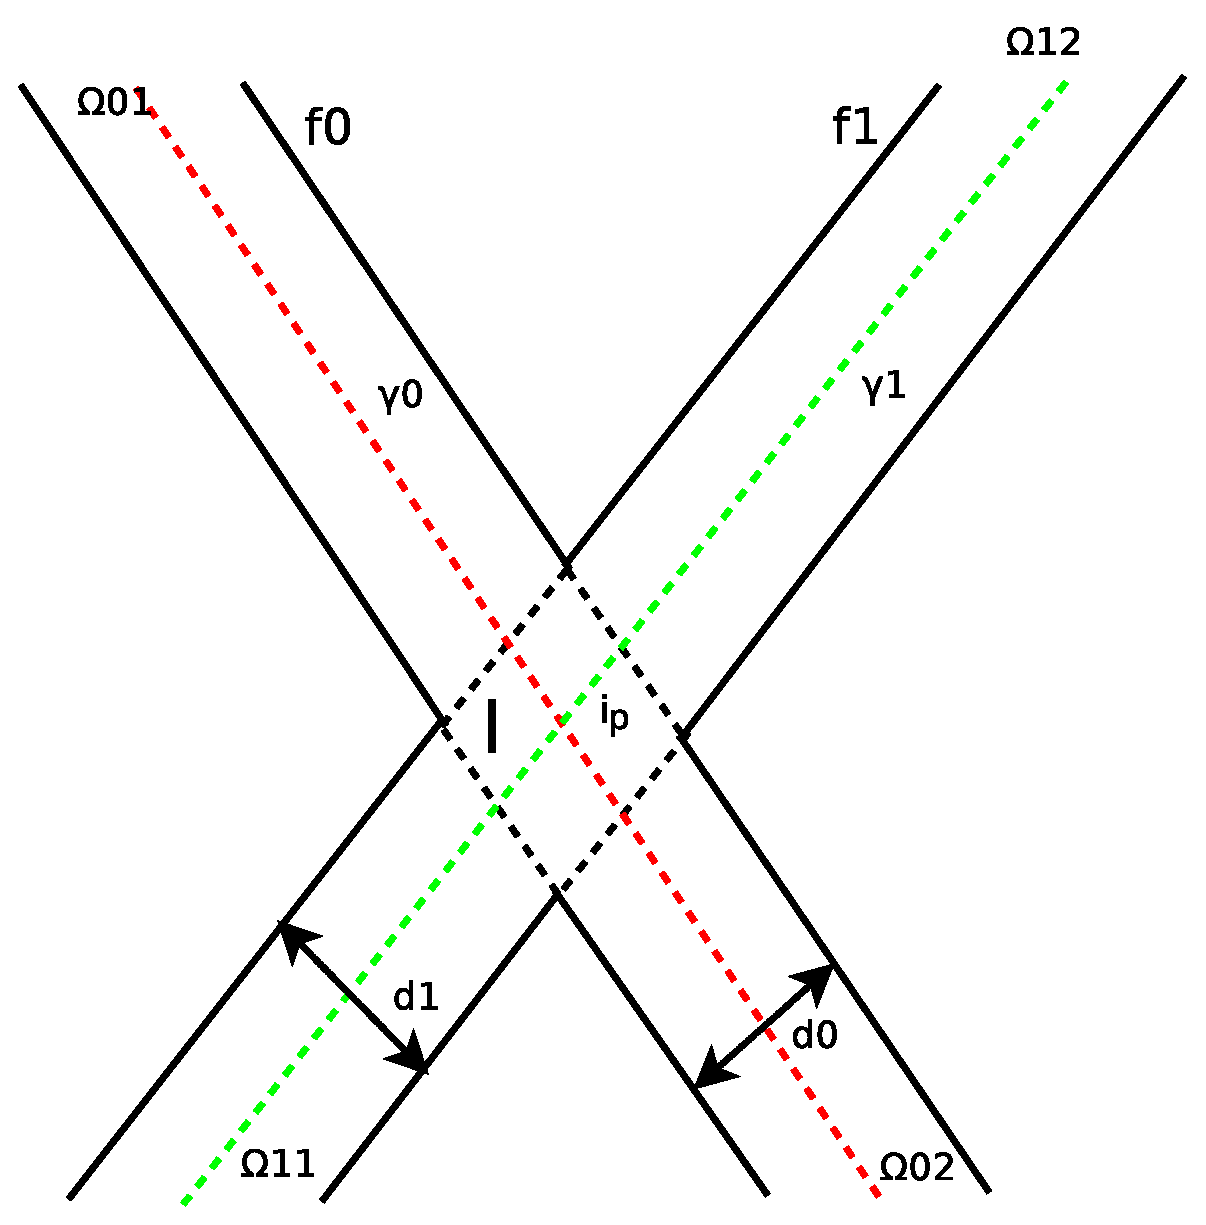
\includegraphics[width=0.4\textwidth]{img/cap2/cross.eps}
\caption{Struttura di un'intersezione di tipo \textit{Cross} tra due fratture.}\label{Cross}
\end{center}
\end{figure}

\noindent L'area di intersezione è constituita da un parallelogramma che suddivide ogni frattura in due zone $\Omega_{i1}$ e $\Omega_{i2}$. Il modello su cui noi ci basiamo riduce la frattura, qui rappresentata in un dominio $\mathbb{R}^{2}$, alla retta di sostegno $\gamma_i$. In questo modo l'intersezione si riduce ad un punto.\\
Il tipo di intersezione su cui ci siamo concentrate noi, invece, ha la seguente forma:

\begin{figure}[htbp]
\begin{center}
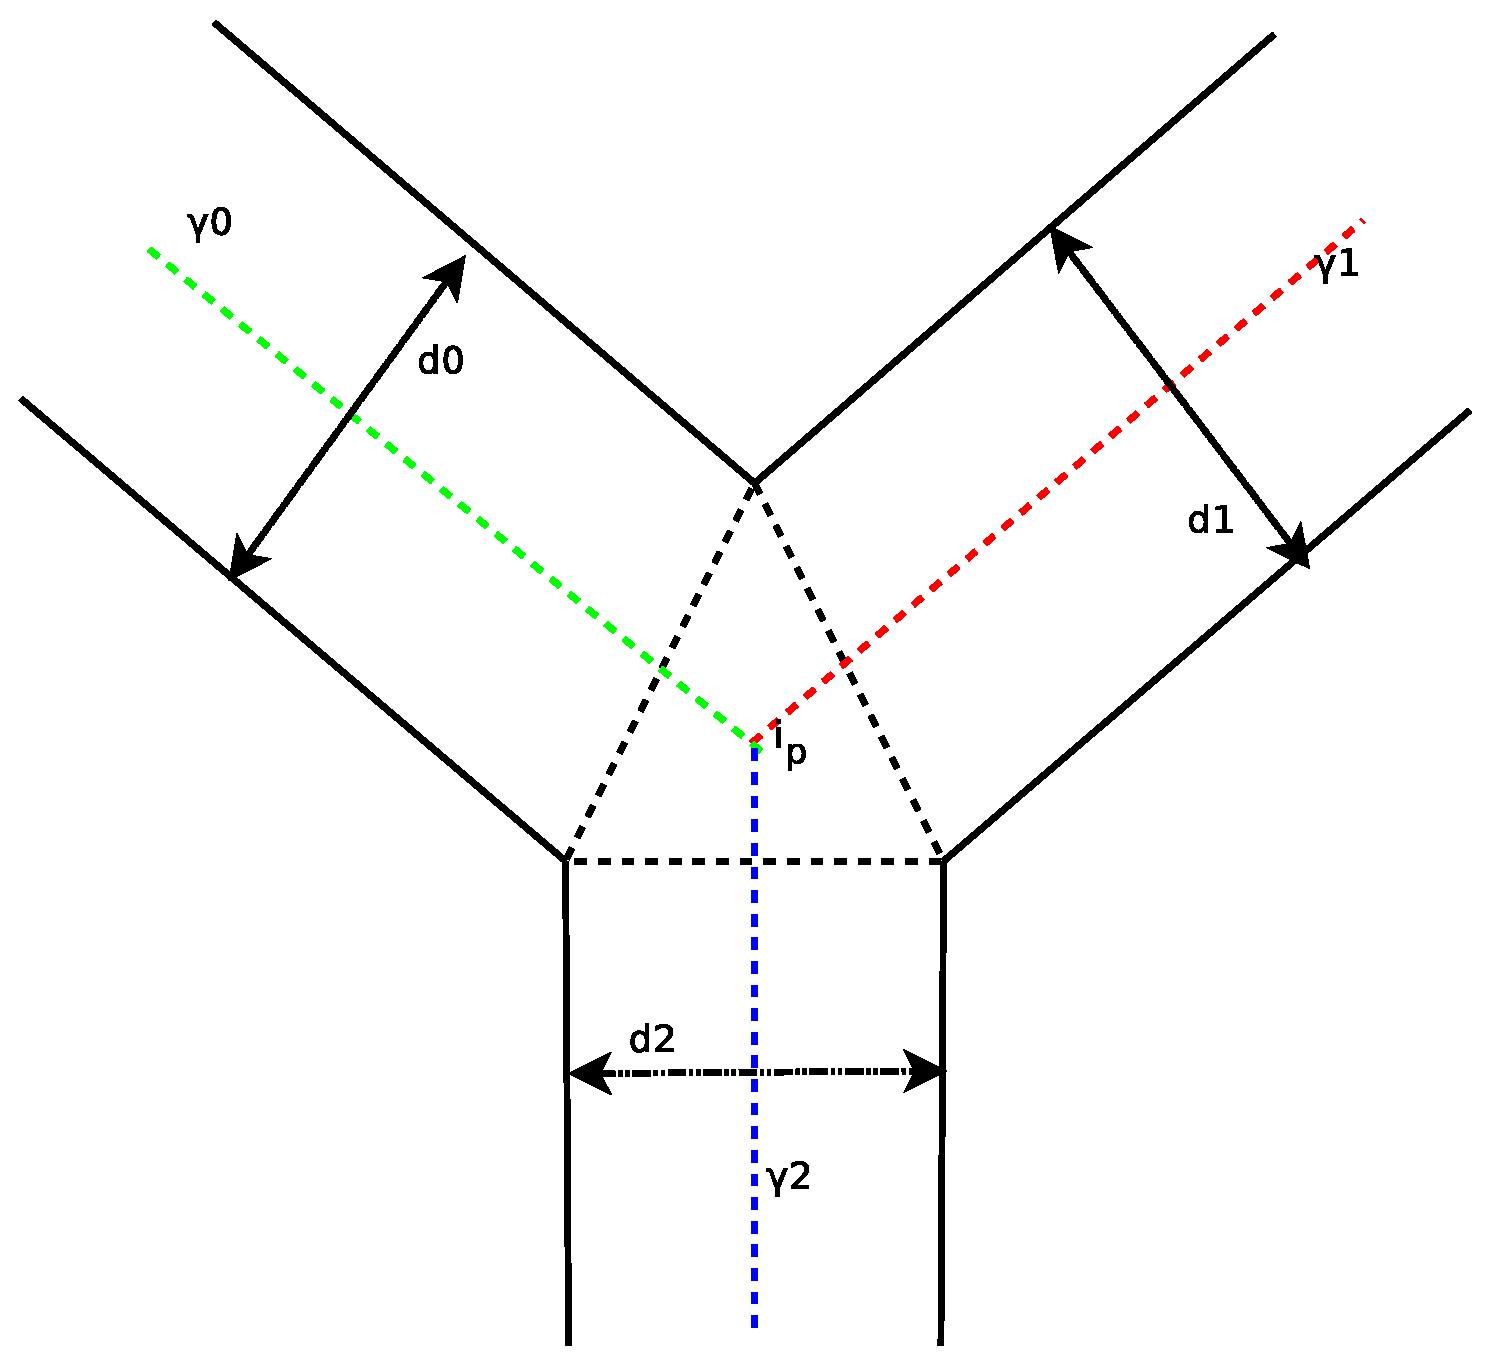
\includegraphics[width=0.4\textwidth]{img/cap2/bifurcation.eps}
\caption{Struttura di un'intersezione di tipo \textit{Bifurcation} tra due fratture.}\label{Bifurcation}
\end{center}
\end{figure}

\noindent In questo caso le fratture coinvolte sono tre e la zona interessata dall'intersezione è rappresentata da un triangolo. Anche qui consideriamo un modello ridotto e le fratture sono individuate dalle rette di sostegno $\gamma_i$ in $\mathbb{R}$. Le condizioni d'interfaccia che vengono ricavate in questo caso valgono solo nel caso in cui le tre fratture si intersechino in un unico punto comune $i_p$ e tale punto sia contenuto nel triangolo d'intersezione nella rappresentazione 2d.

\subsection{File data}

I dati per la definizione del problema sono definiti nei file .txt contenuti nella sottocartella \texttt{dati}. \\
\noindent Ognuno di questi files ha la seguente struttura:

\begin{enumerate}
\item[-] una prima parte dove vengono definite la directory dove trovare l'eventuale mesh da importare, la directory dove salvare i risultati e il numero di fratture che entrano in gioco;
\item[-] una sezione dedicata a parametri e grandezze necessari per la definizione del dominio del mezzo;
\item[-] una sezione per ogni frattura con la dichiarazione del level set, dei parametri che individuano il segmento che rappresenta la frattura e delle grandezze necessarie per risolvere il problema di Darcy.
\end{enumerate}

\begin{Code03_01}[caption={Definizione del dominio}]
meshFile = meshes/mesh		//   directory da cui importare eventualmente la mesh
folderVTK = ./vtk/				//   directory dove salvare i risultati

numberFractures = 3

[mediumData]					//   informazioni legate al mezzo poroso in questione

   [./domain]					//   informazioni necessarie per costruire o importare la mesh 
     [ ... ]
   [../]

   [./darcy]					//   informazioni sulla natura permeabile del mezzo
     invK = 1.
     invKDist11 = 1.
     invKDist12 = 0.
     invKDist22 = 1.
     [...]	
   [../]

[../]

\end{Code03_01}

\par \noindent Nonostante il nostro problema si concentri solamente sulla soluzione del flusso all'interno delle fratture, noi costruiamo comunque la mesh relativa al mezzo. Questa mesh verrà usata solamente come supporto, sarà puramente accessoria nel corso dell'implementazione. \\
 \noindent Per quanto riguarda la permeabilità, poichè le fratture sono costituite dallo stesso materiale, questa resta uguale in tutto il dominio. 

\begin{figure}[htbp]
\begin{center}

\includegraphics[width=0.65\textwidth]{img/cap2/mesh.eps}
\caption{Principali parametri di definizione per una frattura}
\end{center}
\end{figure}

\begin{Code03_01}[caption={Definizione della frattura}]
[fractureData]

spaceDimension = 1.

   [./levelSet]		// parametri di definizione del level set
     // funzione level set che rappresenta la frattura
     levelSet = y-a*x-b 			
     ylevelSet = y-a1*t-b1 			
     xlevelSet = x-a2*t-b2				          
     levelSetCut = -1	
     yMap = a1*t+b1					
     xMap = a2*t+b2				
     // fattore di scala, rapporto tra la lunghezza della mesh di integrazione e la 
     // lunghezza della mesh reale
     jacMap = [ h/h1 ]				
     normalMap = [ ]					
     integrationTypeSimplex = IM_STRUCTURED_COMPOSITE(IM_TRIANGLE(3),1)
   [../]

   [./domain]		// parametri di definizione del dominio di integrazione
     thickness = 
     spacing = x+c      	
     spatialDiscretization = n
     // dimensioni del dominio
     translateAbscissa = c
     lengthAbscissa = h1
     lengthOrdinate = 0.
     lengthQuota = 0.
     meshType = GT_PK(1,1)
     // variabili per l'integrazione
     integrationTypeVelocity = IM_GAUSS1D(3)
     integrationTypePressure = IM_GAUSS1D(2)		
     FEMTypeVelocity = FEM_PK(1,1)
     FEMTypePressure = FEM_PK(1,0)
     FEMTypeLinear = FEM_PK(1,1)
   [../]

   [./darcy]		// parametri per la definizione del problema di Darcy
     etaNormal = 0.01
     etaNormalDistribution = 1. 
     etaTangential = 100.
     etaTangentialDistribution = 1.
     source = 
     solution = 
     velocity = 
   [../]

[../]

\end{Code03_01}


\lstnewenvironment{Code03_01}[1][]{\lstset{basicstyle=\small\ttfamily, columns=fullflexible,framexrightmargin=+.1\textwidth, keywordstyle=\color{red}\bfseries, commentstyle=\color{blue},language=C++, basicstyle=\small,  numberstyle=\tiny, stepnumber=1, numbersep=5pt, frame=shadowbox, #1}}{}


\chapter{Strumenti di sviluppo}
Lo sviluppo della nostra libreria ha richiesto l'uso di strumenti specifici atti a facilitare e sistematizzare la gestione del codice quali \texttt{git}, \texttt{CMake} e \texttt{Dxygen}.\\
\href{https://github.com/}{\texttt{Git}} è un sistema di controllo versione utilizzavile direttamente da linea di comando, molto diffuso è utile per tenere traccia delle varie fasi di sviluppo del codice. Git gestisce in modo adeguato i contributi al codice provenienti da agenti esterni e permette la condivisione del codice.\\
\href{http://www.cmake.org/}{\texttt{CMake}} è un software libero multipiattaforma nato per l'automazione dello sviluppo. Sostanzialmente con l'uso di \texttt{CMake} è possibile configurare e generare Makefile per il sistema operativo in uso. Questo facilita la diffusione del codice tra sviluppatori, non dovendo far altro che lanciare \texttt{CMake} e lasciare che sia lui ad occuparsi della ricerca di compilatori e librerie locali e della costruzione di software.\\
\href{www.doxygen.org/}{\texttt{Doxygen}} è un sistema multipiattaforma molto diffuso per la generazione automatica della documentazione di un codice. Per ottenere la documentazione è necessario introdurre nel codice dei commenti con una sintassi particolare, e il risultato è contiene l’elenco delle classi implementate, i loro diagrammi di collaborazione e la descrizione di metodi ed attributi.

\section{\texttt{Git}}
Il codice del progetto è reperibile su \texttt{git} ed è possibile scaricarlo e collabolare allo sviluppo clonando il codice dalla repository  \href{https://github.com/}{\texttt{GitHub}}:\\
\begin{center}
\texttt{ git clone https://github.com/mariaiemoli/progetto.git}
\end{center}
Nella cartella principale è contenuto anche un file \texttt{.gitignore}, in cui sono specificate le estensioni dei files e le sottocartelle che non devono essere visionati in una repository \texttt{git}. In particolare non si è interessati ai files temporanei che vengono eventualmente generati dagli editor, e alle cartelle generate da uno scorretta configurazione di \texttt{Doxygen}.

\section{\texttt{CMake}}
\texttt{CMake} si basa sulla creazione di files \texttt{CMakeLists.txt} nella directory del progetto, che contengono le direttive necessarie per creare il \texttt{Makefile} per compilare ed eseguire il codice. \\
Nella directory principale si trova un primo file \texttt{CMakeLists.txt} in cui si impostano i parametri fondamentali quali la dipendenza dalla versione di \texttt{CMake}, il nome del progetto, si includono le directory dei sorgenti nel path di compilazione e si caricano le librerie esterne utilizzate dai sorgenti. \\
le librerie che vengono caricate sono:
\begin{itemize}
\item \texttt{Eigen}, libreria template per l'algebra lineare usata principalmente nella fase di imposizione delle condizioni di interfaccia sul triangolo di intersezione nel caso della biforcazione, per il modello ridotto;
\item \texttt{Getfem++}, libreria matematica per gli elementi finiti usata per scrivere e risolvere il problema numerico;
\item \texttt{Blas} (Basic Linear Algebra Subprograms) e \texttt{Qhull}, librerie necessarie per \texttt{Getfem++};
\item \texttt{Doxygen}, usato per generare la documentazione
\end{itemize}

\begin{Code03_01}
CMAKE_MINIMUM_REQUIRED( VERSION 2.8 )

PROJECT(PACS)

SET(CMAKE_CXX_FLAGS "-std=c++0x -Wall ${CMAKE_CXX_FLAGS}")

SET(CMAKE_MODULE_PATH 
	${CMAKE_SOURCE_DIR}/cmake ${CMAKE_MODULE_PATH})

# Include Eigen3
FIND_PACKAGE(PkgConfig)
PKG_CHECK_MODULES(EIGEN3 REQUIRED eigen3)
INCLUDE_DIRECTORIES(${EIGEN3_INCLUDE_DIRS})

# Include Doxygen
find_package(Doxygen)
[ ... ]

# Include Getfem
if (GETFEM_LIBRARIES AND GETFEM_INCLUDE_DIRS)
[ ... ]

#Include for BLAS library
find_package ( BLAS )
[ ... ]


#Include for LAPACK library
find_package ( LAPACK )
[ ... ]

#Include for QHULL library
set(QHULL_MAJOR_VERSION 6)
[ ... ]

SET(CMAKE_INSTALL_PREFIX 
	${CMAKE_SOURCE_DIR}/install-dir CACHE PATH "" FORCE)

ADD_SUBDIRECTORY(src)
ADD_SUBDIRECTORY(test)
\end{Code03_01}

Per poter usare \texttt{CMake} è necessario posizionarsi nella directory in cui è contenuto il progetto e creare una cartella in cui compilare il codice. Per lanciare \texttt{CMake} è necessario digitare i seguenti comandi: \\ 
%\begin{center}
 \texttt{cd $<$build\_dir$>$ } \\
\texttt{cmake $<$source\_dir$>$}
%\end{center}

\texttt{CMake} imposta le variabili di path come definito nel file  \texttt{CMakeLists.txt}, esamina le dipendenze da librerie esterne e procede esaminando le sottocartelle aggiunte nel file di configurazione. In particolare esamina le sottocartelle \texttt{src} e \texttt{test}, in cui sono presenti altri files  \texttt{CMakeLists.txt}, che impostano i rispettivi obiettivi e definiscono le rispettive sottocartelle. Questo permette a \texttt{CMake} di esaminare tutta la directory in cui è contenuto il progetto in maniera ricorsiva. \\
Nella cartella \texttt{src} il file  \texttt{CMakeLists.txt} aggiunge la creazione di una libreria a partire dal codice del progetto. 
\begin{Code03_01}
ADD_LIBRARY(pacs ${TARGET_SRC} ${TARGET_HANDLER})
\end{Code03_01}

Nella cartella test si trovano dei files data di esempio per poter eseguire il codice, contenuti della sottocartella \texttt{data}. Il file  \texttt{CMakeLists.txt} nella cartella dei test definisce gli obiettivi e i collegamenti necessari per l'esecuzione. 

\par Una volta che il \texttt{Makefile} è stato generato è possibile compilare il codice con il comando: \\ 
\texttt{make}.
Questo crea nella sottocartella \texttt{test} un eseguibile chiamato \texttt{darcy}. Per poterlo eseguire è sufficiente lanciarlo da terminale dandogli in pasto uno dei files presenti nella sottocartella \texttt{data}:\\
\texttt{ .\textbackslash darcy data\textbackslash$<$file\_data$>$ }

\section{\texttt{Doxygen}}
Per poter creare la documentazione al codice con \texttt{Doxygen} è necessario che nella cartella principale sia presente il file \texttt{Doxygen}, in caso contrario è necessario crearlo con il comando:\\
\texttt{Doxygen -g}\\
In questo file sono definite le variabili che permettono di creare la documentazione come il nome del progetto, la directory dove creare la documentazione, le cartelle dove si trovano i sorgenti e l'estensione dei files da considerare.

\begin{Code03_01}
PROJECT_NAME 				=	 Problema di Darcy in un network di fratture
OUTPUT_DIRECTORY			=	./build/doc
INPUT						= 	./src ./test
FILE_PATTERNS				= 	*.cc *.h
HAVE_DOT					=	YES
COLLABORATION_GRAPH		=	YES
HIDE_UNDOC_RELATIONS		=	NO
\end{Code03_01}

Dopo aver lanciato \texttt{CMake} è possibile generare la documentazione semplicemente eseguendo: \\
\texttt{cd $<$build\_dir$>$} \\
\texttt{make doc}

Questo crea una sottocartella \texttt{build/doc} che contiene la documentazione \texttt{html} e \LaTeX{}.
\chapter{Problema numerico}
\section{Descrizione dello scenario}
\lstnewenvironment{Code03_03}[1][]{\lstset{basicstyle=\small\ttfamily, columns=fullflexible,framexrightmargin=+.1\textwidth, keywordstyle=\color{red}\bfseries, commentstyle=\color{blue},language=C++, basicstyle=\small, numbers=left, numberstyle=\tiny, stepnumber=1, numbersep=5pt, frame=shadowbox, #1}}{}

\chapter{Classi per la gestione del problema numerico}
\section{Class BC}
\subsection{Definizione della classe e costruttore}
La classe \texttt{BC} ci permette di introdurre le condizioni al bordo. Viene gestito sia il bordo del 		mezzo, che quello di ogni singola frattura. \\ 
Il suo costruttore richiede i seguenti parametri:
	\begin{itemize}
	\item \textit{Mesh:} relativa al mezzo o a una delle fratture
	\item \textit{Stringa:} contenente il tipo di mesh di GetFem del elemento precedente
	\item \textit{Vettore:} nullo, se la mesh fa riferimento al mezzo, contenete gli indici dei gradi di libert\`{a} degli estremi, se si sta lavorando su una frattura
	\item \textit{ElementDimesion:} dimensione in cui stiamo lavorando ( di defaul 2 per il mezzo e 1 per le fratture)
	\end{itemize}
e crea un elemento \texttt{BC} formato da:
	\begin{itemize}
	\item \textit{Mesh:} relativa al mezzo o a una delle fratture
	\item \textit{Vettore:} contenente l'indice dei gradi di libert\'{a} in cui è imposto Dirichlet
	\item \textit{Vettore:} contenente l'indice dei gradi di libert\'{a} in cui è imposto Newmann
	\item \textit{Vettore:} contenente l'indice dei gradi di libert\'{a} in cui sono imposte le condizioni al bordo
	\end{itemize} 

\newpage	
\begin{Code03_03}[caption={Classe \texttt{BC}}]
public:

    enum
    {
        DIRICHLET_BOUNDARY_NUM = 40,
        NEUMANN_BOUNDARY_NUM = 50
    };

    // Costruttore
    BC ( getfem::mesh& mesh,
         const std::string& MeshType,
         const sizeVector_Type DOFs,
         const ElementDimension& dimension = MEDIUM );

private:

    getfem::mesh_fem M_meshFEM;
    
    // flags for BC
    sizeVector_Type M_dirichlet;
    sizeVector_Type M_neumann;
    sizeVector_Type M_extBoundary;
\end{Code03_03}

\begin{Code03_03}[caption={Typedef per la Classe \texttt{BC}}]
/*! Elemento BC */
typedef BC BC_Type;
/*! Puntatore alla classe BC */												
typedef boost::shared_ptr<BC> BCPtr_Type;
/*! Vettore di puntatori a BC */			
typedef std::vector<BCPtr_Type> BCPtrContainer_Type;	
\end{Code03_03}

Sia quando lavoriamo sul dominio del mezzo, che quando stiamo considerando una frattura che ha solo intersezioni di tipo cross con le altre, il costruttore andrà a inserire gli indici dei gradi di libert\`{a} nei rispettivi vettori valutando solamente se essi si trovano su una faccia della mesh.
Nel caso della biforcazione bisogna accertarsi di imporre le condizioni al bordo solamente nel'estremo libero, ovvero quello in cui non v\`{e} l'intersezione delle tre fratture.

\subsection{Novit\`{a} introdotte per la biforcazione}
Quando andiamo ad analizzare una frattura è dunque necessario fornire al costruttore il vettore dei DOF liberi e imporre le condizioni solamente nel DOF dove v\`{e} intersezione. Per far questo creiamo un variabile booleana che varr\`{a} 1 se il grado di libert\`{a} che sto considerando è contenuto nel vettore dei DOF liberi, 0 altrimenti. Questo mi permette di inserire un controllo prima di aggiungere quel indice ai campi \texttt{M\_dirichlet} , \texttt{M\_neumann} , \texttt{M\_extBoundary} della classe.
%PER MERY -> uso " vettore dei DOF liberi " senza spiegarlo perchè mi aspetto l'abbia spiegato tu quando spieghi il campo di Fracture Handler
\begin{Code03_03}[caption={Classe \texttt{BC}}]
[...]

getfem::mesh_region borderFaces;
getfem::outer_faces_of_mesh(mesh, borderFaces);

[...]
/* Boundary e' un size_type che contine la cardinalita' dei DOF 
 * appartenti alle faccie della mesh */
 
boundary_cv.resize(Boundary);
boundary_flags.resize(Boundary);

for ( getfem::mr_visitor i(borderFaces); !i.finished(); ++i )
{
	bool ImAnIntersectionDOF = 0;
				
	for( size_type j=0; j<DOFs.size(); j++ )
	{
		if( DOFs[ j ] == i.cv() )
		{
			ImAnIntersectionDOF = 1;
		}
	}
	if ( !ImAnIntersectionDOF )
	{
	  if (false)//( gmm::abs(gmm::abs(un [ dimension - 1 ]) - 1.0) > 1.0E-7 )  
	  {				
		// Dirichlet, flag 0
		boundary_cv [ i.cv() ].push_back(i.f());
		boundary_flags [ i.cv() ].push_back(boundaryFlags [ 1 ]);
		
	  }
	  else
	  {
		// Neumann, flag 1
		boundary_cv [ i.cv() ].push_back(i.f());
		boundary_flags [ i.cv() ].push_back(boundaryFlags [1 ]);
	  }
	}
}

[...]
\end{Code03_03}



\section{Class BCHandler}

Work in progress

\section{Class DarcyFracture}

Work in progress


\lstnewenvironment{Code03_04}[1][]{\lstset{basicstyle=\small\ttfamily, columns=fullflexible,framexrightmargin=+.1\textwidth, keywordstyle=\color{red}\bfseries, commentstyle=\color{blue},language=C++, basicstyle=\small, numbers=left, numberstyle=\tiny, stepnumber=1, numbersep=5pt, frame=shadowbox, #1}}{}

\chapter{Classi per la gestione del problema numerico}

\section{Class \texttt{DarcyFracture}}
La classe \texttt{DarcyFracture} ci permette di passare alla formulazione algebrica, $ Ax=b $, del problema e di risolverlo. \\ 

%Il suo costruttore richiede i seguenti parametri:
%	\begin{itemize}
%	\item \textit{Mesh:} relativa al mezzo o a una delle fratture
%	\item \textit{Stringa:} contenente il tipo di mesh di GetFem del elemento precedente
%	\item \textit{Vettore:} nullo, se la mesh fa riferimento al mezzo, contenete gli indici dei gradi di libert\`{a} degli estremi, se si sta lavorando su una frattura
%	\item \textit{ElementDimesion:} dimensione in cui stiamo lavorando ( di defaul 2 per il mezzo e 1 per le fratture)
%	\end{itemize}
I campi fondamentali della classe sono:
	\begin{enumerate}
	\item[-] \texttt{M\_globalMatrix}: \`{e} una matrice a blocchi sparsa rappresentata i GETfem da un \textit{boost::shared\_ptr $\langle$ gmm::row\_matrix $\langle$ sparseVector\_Type $\rangle \rangle$};
	\item[-] \texttt{M\_globalRightHandSide}: vettore del termine noto;
	\item[-] \texttt{M\_velocityAndPressure}: vettore soluzione delle velocit\'{a} e della pressione.
	\end{enumerate} 

\begin{Code03_04}[caption={Classe \texttt{DarcyFracture}}]
class DarcyFractured
{
 public:
    DarcyFractured ( const MediumDataPtr_Type& medium,
                     const MeshHandlerPtr_Type& mesh,
                     const BCHandlerPtr_Type& bcHandler,
                     const FracturesSetPtr_Type& fractures,
                     const ExporterPtr_Type& exporter );
    
    void init ( );
    
    void assembly ( const GetPot& dataFile );

    void solve ( );

	[ ... ]

 private:

	[ ... ]

    sparseMatrixPtr_Type M_globalMatrix;

    scalarVectorPtr_Type M_globalRightHandSide;

    scalarVectorPtr_Type M_velocityAndPressure;

    [ ... ]
};
\end{Code03_04}

Il metodo init() setta tutte le costanti note del problema.
Il metodo assembly() crea la matrice globale $A$ e il termine noto di destra, utilizzando le funzioni della classe \texttt{XFEMOperators}. 
Ipotizzando di avere un ambiente dove tre fratture hanno un intersezione di tipo \textit{Bifurcation} e una di queste si incontra con una quarta creando un intersezione di tipo \textit{Cross}, la matrice globale avrà il seguente volto:\\
%---->DA SISTEMAREEEEE <----------------- 
 \begin{center}
  $ \left[ \begin{matrix}
 			A_{0} &  B_{0} & 0 & 0 & 0 & 0 & 0 & 0 & 0\\ 
 			B_{0}^{T} & 0 & 0 & 0 & 0 & 0 & 0 & 0 & 0\\
 			0 & 0 & A_{1} &  B_{1} & 0 & 0 & 0 & 0 & 0 \\ 
		 	0 & 0 & B_{1}^{T} & 0 & 0 & 0 & 0 & 0 & 0 \\
		 	0 & 0 & 0 & 0 & A_{2} &  B_{2} & 0 & 0 & E_{2} \\ 
		 	E_{2}^{T} & 0 & 0 & 0 & B_{2}^{T} & 0 & 0 & 0 & 0\\
		 	0 & 0 & 0 & 0 & 0 & 0 & A_{3} &  B_{3} & E_{3} \\ 
 			E_{3}^{T} & 0 & 0 & 0 & 0 & 0 & B_{3}^{T} & 0 & 0\\
 			0 & 0 & 0 & 0 & E_{2}^{T} & 0 & E_{3}^{T} & 0 & 0\\
 			\end{matrix}.\right] $ 
  \end{center}
Nel caso di un \textit{Cross} le matrici $E_{2}$ e $E_{3}$, generate durante l'assembly(), impongonole condizioni di interfaccia in maniera debole .\\
Nel caso di una \textit{Bifurcation} prima di terminare la funzione assembly() impone in maniera forte le condizioni di interfaccia, ricavate con il confronto col mondo 2D, nella riga corrispondente al DOF di pressione e di velocit\`{a} relativo al punto d' intersezione della frattura.\\
Infine il metodo solve() risolve il problema e esporta i risultati ottenuti in formato \emph{vtk} per entrambe le incognite.\\

%\section{Class \texttt{XFEMOperetors}}
%Ogni frattura ha associata la matrice:
%\begin{center} 
% $ \left[ \begin{matrix}
% 	A11 &  A12 \\ 
% 	A12^{T} & 0
% \end{matrix}\right] $
%\end{center} 
%
%La classe \texttt{XFEMOperators} implementa le funzioni che ci permettono di calcolare questi blocchi.
%Le sue funzioni principali sono le seguenti:
%
%\begin{Code03_03}[caption={Funzioni per assemblare la matrice globale}]
%//Costruisce  A11 = Aij = a(\phi_j, \phi_i)
%void darcy_A11F ( sparseMatrixPtr_Type& M,
%                  const FractureHandlerPtr_Type& fracture,
%                  const scalar_type& gammaU,
%                  const scalarVector_Type& invKTangentialInterpolated,
%                  const sizeVector_Type &ExtBoundary,
%                  const size_type& uncutRegionFlag );
%
%// Aggiorna A11 nel caso intersezione" Cross "
%void darcy_A11F_Cross ( sparseMatrixPtr_Type& M,
%					    const FractureHandlerPtr_Type& fracture,
%					    const scalarVector_Type& invKTangentialInterpolated,
%					    const FractureHandlerPtr_Type& otherFracture,
%					    const size_type& cutRegionFlag );
%
%//Costruisce A12 = Bij = b(\phi_j, \omega_i)
%void darcy_A12F ( sparseMatrixPtr_Type& M,
%                  const FractureHandlerPtr_Type& fracture,
%                  const size_type& uncutRegionFlag );
%
%//Aggiorna A12 = Bij = b(\phi_j, \omega_i) nel caso di intersezione " Cross "
%void darcy_A12F_Cross ( sparseMatrixPtr_Type& M,
%                  	    const FractureHandlerPtr_Type& fracture,
%                  	    const FractureHandlerPtr_Type& otherFracture,
%                  	    const size_type& cutRegionFlag );
%\end{Code03_03}
%
%Altre importanti funzioni sono quelle che ci permetto di costruire il termine noto e son sempre contenute in questa classe.

\chapter{Il caso Unicredit - titolo provvisorio} 

La realtà in analisi è un grosso gruppo finanziario internazionale. L'ambiente
progettato e realizzato durante il mio stage aziendale elabora i
dati di circa 90000 dipendenti dell'azienda, ed è predisposto per gestirne
altrettanti aggiuntivi, alla luce di una grossa fusione avvenuta di recente.
Il sistema di gestione delle identità realizzato è subentrato gradualmente
all'architettura precedentemente esistente e, di conseguenza, la sua
progettazione ha dovuto considerare la possibilità di
inserimento graduale nel ciclo di vita di tutto il resto dell'architettura
aziendale.

Subentrare ad una realtà già esistente è stato un notevole vantaggio perchè ha
permesso di analizzare quanto già creato e migliorare i difetti più evidenti
mantenendone i punti di forza.

\section{Ambiente AS-IS}

\begin{sidewaysfigure}[tbp]
\centering
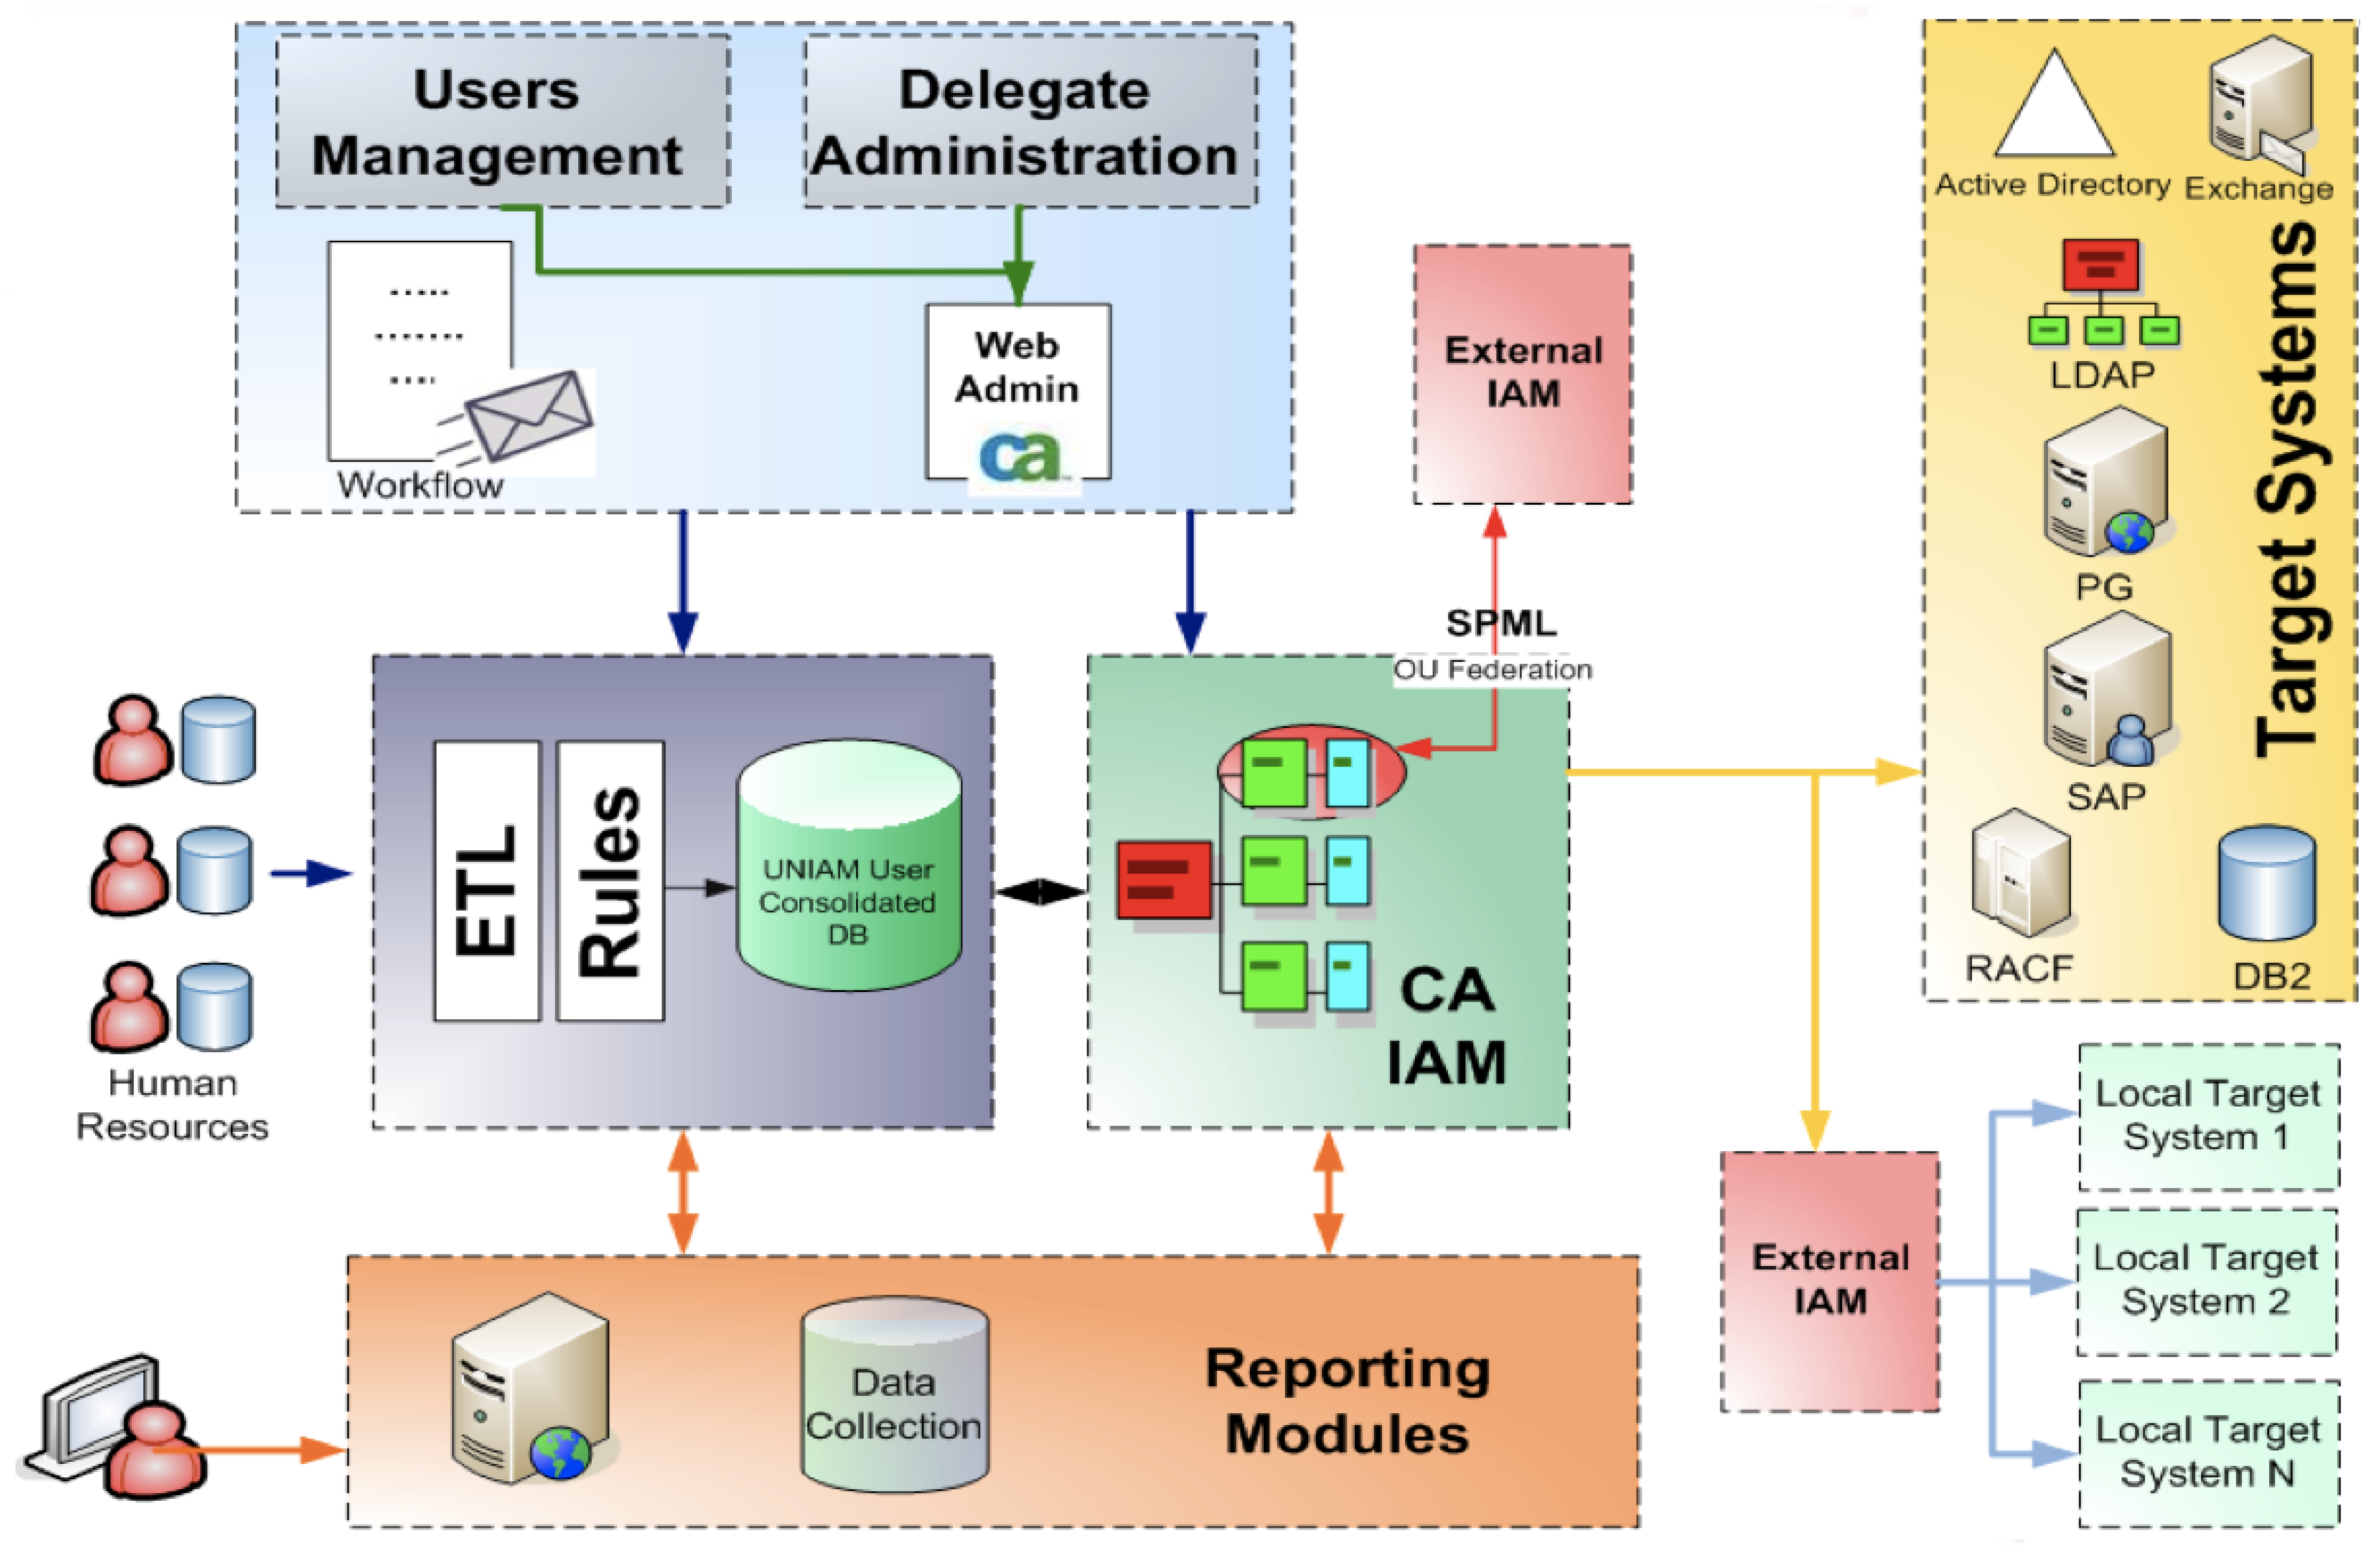
\includegraphics[width=0.95\textwidth]{img/soluzioneCA.eps}
\caption{Architettura IAM}
\label{soluzioneCA}
\end{sidewaysfigure}

In figura\ref{soluzioneCA} è illustrata la soluzione completa attualmente
funzionante. La maggior parte delle componenti di IAM presenti è implementata
con prodotti di Computer Associates~\footnote{CA - http://www.ca.com}.

Il sistema si occupa della gestione del personale di quasi tutto il gruppo
bancario. Alcune banche e assicurazioni controllate non sono state ancora
inserite, benchè la loro integrazione sia prevista entro la fine del 2009.
Un'immagine rappresentativa delle prestazioni ottenute è rappresentata in
figura~\ref{descrizioneprogetto}


\begin{sidewaysfigure}[tbp]
\centering
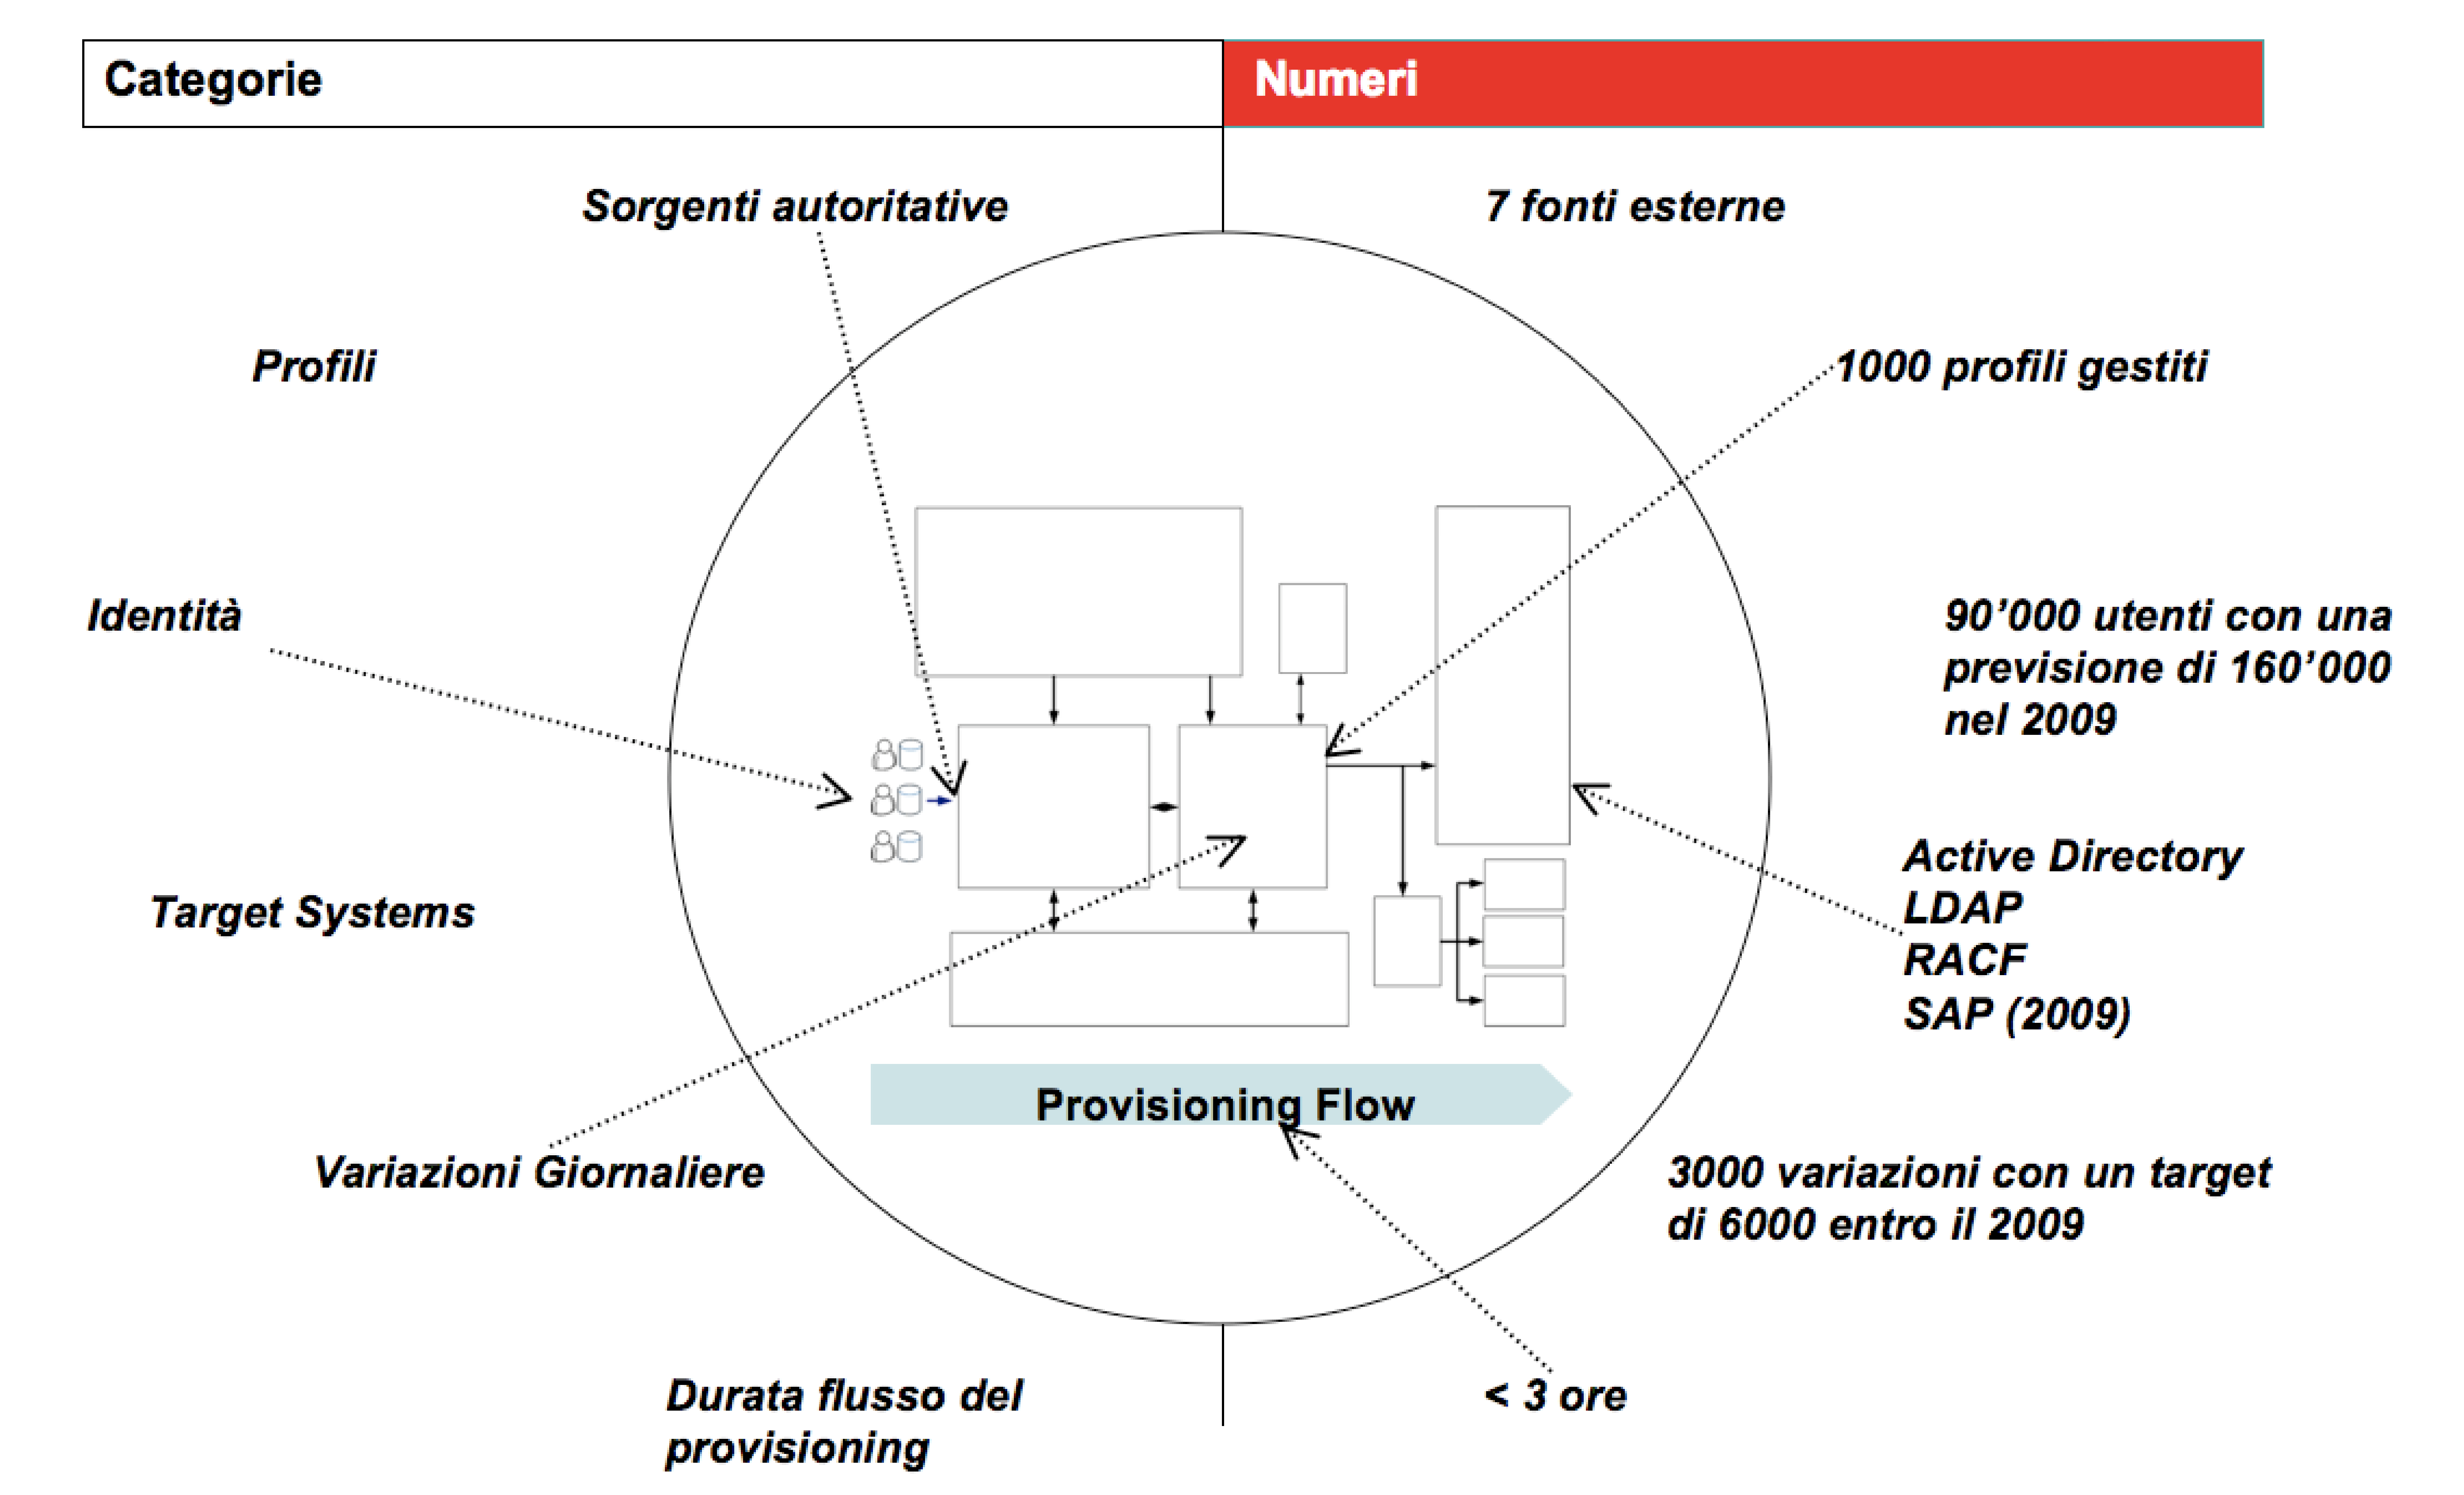
\includegraphics[width=0.95\textwidth]{img/descrizioneprogetto.eps}
\caption{Ordine di grandezza dei dati trattati}
\label{descrizioneprogetto}
\end{sidewaysfigure}

La gestione delle utenze avviene a partire da quanto presente nei data base
degli uffici del personale (HR). 
L'ufficio HR inserisce per ogni dipendente un profilo contenente tutte le
informazioni necessarie in base alle policy della singola azienda in un data
base. Normalmente i DB utilizzati sono ospitati su mainframe e principalmente
sono di tipo DB2~\cite{DB2}, anche se alcune fonti usano SQL server
2005~\cite{SQLServer2005} e perfino flat file.
Le basi di dati vengono denominate \textit{fonti autoritative}, per evidenziarne
il ruolo chiave che questi dati rivestono ai fini della definizione del profilo utente. 
La soluzione implementata comporta il minor impatto possibile sulla struttura
già presente in tutte le realtà che compongono il gruppo finanziario, nella
totalità dei casi ci si limita a leggere i dati forniti senza apportare alcuna
modifica alla sorgente.
I dati letti dalle sorgenti vengono elaborati dal nucleo del sistema di IAM,
componente che è stato reingenierizzato durante lo stage di laurea, e vengono
generate delle istruzioni di modifica del profilo utente in relazione alla
situazione consolidata dell'esecuzione precedente. Queste istruzioni comportano
delle sequenze di comandi sui profili degli utenti, che consistono in operazioni
di cancellazione, modifica o aggiunta di attributi. 
Le istruzioni e il meccanismo di modifica del profilo verrà trattato
approfonditamente nel seguito della relazione.
Il sistema target di tutte le azioni di modifica è un directory LDAP~\cite{LDAP}
che contiene un sottoalbero per ogni utente del sistema, la modifica di un
attributo comporta una serie di operazioni che vengono portate a termine sui
server in produzione, configurando l'immagine di ogni utente come richiesto dal
sistema di IAM.
La scelta di avere un server LDAP come interfaccia tra lo IAM e i sistemi target
è molto utile perchè permette di rendere indipendenti i due ambienti. Alla luce
di questa decisione implementativa è risultato facile sostituire il blocco
dell'ETL custom precedentemente in essere con una soluzione diversa senza
rompere l'equilibrio degli altri componenti dell'architettura.

Il nucleo del framework di IAM è composto da tre macro-componenti che
svolgono, ciascuna, una parte delle elaborazioni necessarie per portare a
termine in modo efficace ed efficiente l’interno processo di provisioning delle
identità e di gestione degli accessi:

\begin{itemize}
\item \textbf{ETL}: la componente di ETL (Extract, Transform, Load) si occupa
dell’estrazione, trasformazione e caricamento dei dati in un sistema di sintesi.
I dati vengono estratti da sorgenti quali database transazionali (DB2, SQL
Server), comuni file di testo (presenti in locale o prelevati da sistemi remoti)
o da altri sistemi informatici che forniscono le informazioni raccolte dai
sistemi di HR (Human Resource).
I dati prelevati subiscono quindi un processo di trasformazione, che consente ad
esempio di selezionare solo quelli che sono di interesse per il sistema,
normalizzare i dati, derivare nuovi parametri, cercare correlazioni tra
dati recuperati da differenti tabelle, etc.
Tale trasformazione ha lo scopo di rendere omogenei dati provenienti da sorgenti
diverse e di fare in modo che siano più aderenti alla logica di business del
sistema per cui viene sviluppato il processo di provisioning. 
L’ultima operazione svolta dalla componente ETL è quella di determinare le
variazioni presenti sui profili normalizzati rispetto alla situazione presente
in Admin e consolidata in precedenza. 

\item \textbf{Transaction}: la componente di Transaction ha il compito di prelevare le
informazioni generate dal modulo ETL e di procedere con l’aggiornamento dei profili
utente presenti in Admin applicando le trasformazioni indicate, così da
allineare il profilo utente su Admin con la situazione fornita dai sistemi di
HR.

\item \textbf{Admin}: eTrust Admin è una soluzione robusta e scalabile per il
provisioning di utenti tra molteplici ed eterogenei sistemi (Active
Directory, LDAP, RACF, etc.). Questo meccanismo consente, attraverso una corretta
configurazione di policy, la creazione, la modifica o la rimozione degli utenti
e dei relative oggetti sui diversi sistemi di un organizzazione.
Il vantaggio offerto da questa soluzione è che astrae i sistemi target,
presentando le principali caratteristiche in formato LDAP.
\end{itemize}
  
Mentre l’ultima componente, eTrust Admin, è un prodotto commerciale di
Computer Associates installato e configurato in modo appropriato, le prime due
sono frutto di attività di analisi, progettazione e implementazione svolte
appositamente per l’ambiente presente in azienda.

La parte di cui mi sono occupato principalmente riguarda il modulo di
ETL perché è la parte che più rappresentava un problema in termini di
prestazioni e scalabilità di tutta l'architettura esistente.
Quella che segue è una disamina dettagliata del processo eseguito da ETL e
Transaction, ovvero dalle due componenti custom dell’infrastruttura IAM in
questione.  

\subsection{Soluzione precedente}
Il modulo ETL è stato implementato con del codice custom, realizzato da un
gruppo di programmatori Java e progettato per lavorare strettamente con eTrust
admin attraverso l'interfacciamento LDAP.
Lo stato del sistema target era mantenuto mediante l'ausilio di un database di
appoggio di tipo INGRES~\cite{ingres}, in cui era memorizzato un record per ogni
utente e un hash che identificasse lo stato di ogni riga.
Lo pseudocodice è presentato nel listato~\ref{codicejava}, e descrive le
operazioni di elaborazione effettuate per ogni fonte autoritativa.

\begin{algorithm}
%\dontprintsemicolon

Connessione alla fonte autoritativa\;

\While{esistono utenti non elaborati}{
    Estrai tutte le informazioni presenti\;
    Normalizza il profilo rispetto al consolidato \;
    Applica le policy e ricava i privilegi \;
    Calcola Hash \;
    \If{Hash != Hash consolidato}
    {
        ModificaProfiloLDAP(ProfiloUtente)\;
        \If{Modifica\_riuscita}{
	ConsolidaProfilo \;
	}
    }
}
\label{codicejava}
\caption{Soluzione di ETL precedente}
\end{algorithm}

La trasformazione così implementata presenta diversi punti deboli e
inefficienze, che si è cercato di risolvere con la nuova implementazione:

\begin{enumerate}
\item La soluzione non è scalabile
\item Il codice è difficilmente riutilizzabile, vista la diversa natura delle
sorgenti
\item Non c'è una correlazione forte tra quanto presente nel directory di admin
e l'immagine consolidata dell'utente
\item Il codice è difficilmente manutenibile perchè la curva di apprendimento è
troppo ripida
\item Non è possibile dividere il calcolo delle modifiche e l'esecuzioni delle
operazioni in fasi distinte
\item Eventuali errori di acquisizione dei dati possono portare a modifiche
massive e indesiderate dei profili utente
\item \'E prevista solo un'esecuzione di tipo batch notturna, quando i dati non
vengono modificati
\end{enumerate}

Il raddoppio della base di utenza è stato il motivo principale che ha spinto il
passaggio dal meccanismo sopra descritto a uno più flessibile, che garantisse
degli standard di scalabilità e manutenibilità in linea con il resto
dell'architettura di IAM. 
Un altro punto debole significativo è la resistenza a errori nei dati in
ingresso. Potrebbe potenzialmente capitare (ed è capitato) che delle mancanze di
dati nelle sorgenti scatenassero processi di rimozione massiva indesiderata di
profili utente dai sistemi target, comportando fastidiosi disservizi.

\section{Nuova implementazione del modulo ETL}

Come introdotto poco sopra, il compito della componente di ETL è quello di
prelevare i dati provenienti da HR sotto forme e da sorgenti diverse per poi
procedere con la loro normalizzazione, il completamento degli stessi con
informazioni prelevate da tabelle aggiuntive, la rilevazione delle modifiche
sui profili utente e la generazione dell’input necessario alla Transaction per
allineare, su Admin, i profili degli utenti rilevati come modificati.   
Tutte queste operazioni devono essere fatte rispettando dei vincoli di tempo e
in modo parallelo, riducendo al minimo (possibilmenete eliminando) gli svantaggi
dell'architettura precedentemente in essere.

Lo strumento scelto come base di tutto l'ETL è SQL Server Integration
Services~\cite{SSIS}, che consiste in un modulo integrato in Visual Studio per
elaborare dati provenienti da data base.
Il prodotto in questione risulta essere molto comodo perchè permette agilmente
di:

\begin{itemize}
\item Trattare sorgenti eterogenee (file, DB2, fogli excel, SQL server) in modo
omogeneo
\item Lavorare in modo visuale sui dati 
\item Utilizzare il linguaggio SQL (Transaction-SQL) quando necessario
\item Compiere elaborazioni complesse usando dei linguaggi di programmazione
(Vb.net, VBS)
\end{itemize}

A parte la propaganda commerciale che, si sa, spesso lascia il tempo che trova,
SSIS si è dimostrato essere uno strumento robusto e affidabile, che ha davvero
reso facile l'implementazione della logica applicativa.
Lavorare sui dati ingresso sempre sotto forma di tuple e con gli strumenti
tipici del data mining ha permesso inoltre di avere delle performance molto
buone in termini di tempo di elaborazione e soprattutto ha permesso di mantenere
il codice dell'applicazione spesso immediato da capire.

In figura\ref{nuovaimplementazione} si può vedere lo schema logico di lavoro
della nuova implementazione del modulo ETL. 

\begin{figure}[htbp]
\centering
\includegraphics[width=0.95\textwidth]{img/nuovaimplementazione.eps}
\caption{Flusso logico ETL}
\label{nuovaimplementazione}
\end{figure}


\subsection{Concorrenza nell'accesso ai dati}
\subsection{Scalabilità}


% vim: tw=80 syntax=tex

\section{Caso particolare: biforcazione con due fratture}

Come ultimo caso di studio ci siamo concentrate sulla biforcazione generata da due fratture. 

\begin{figure}[htbp]
\begin{center}
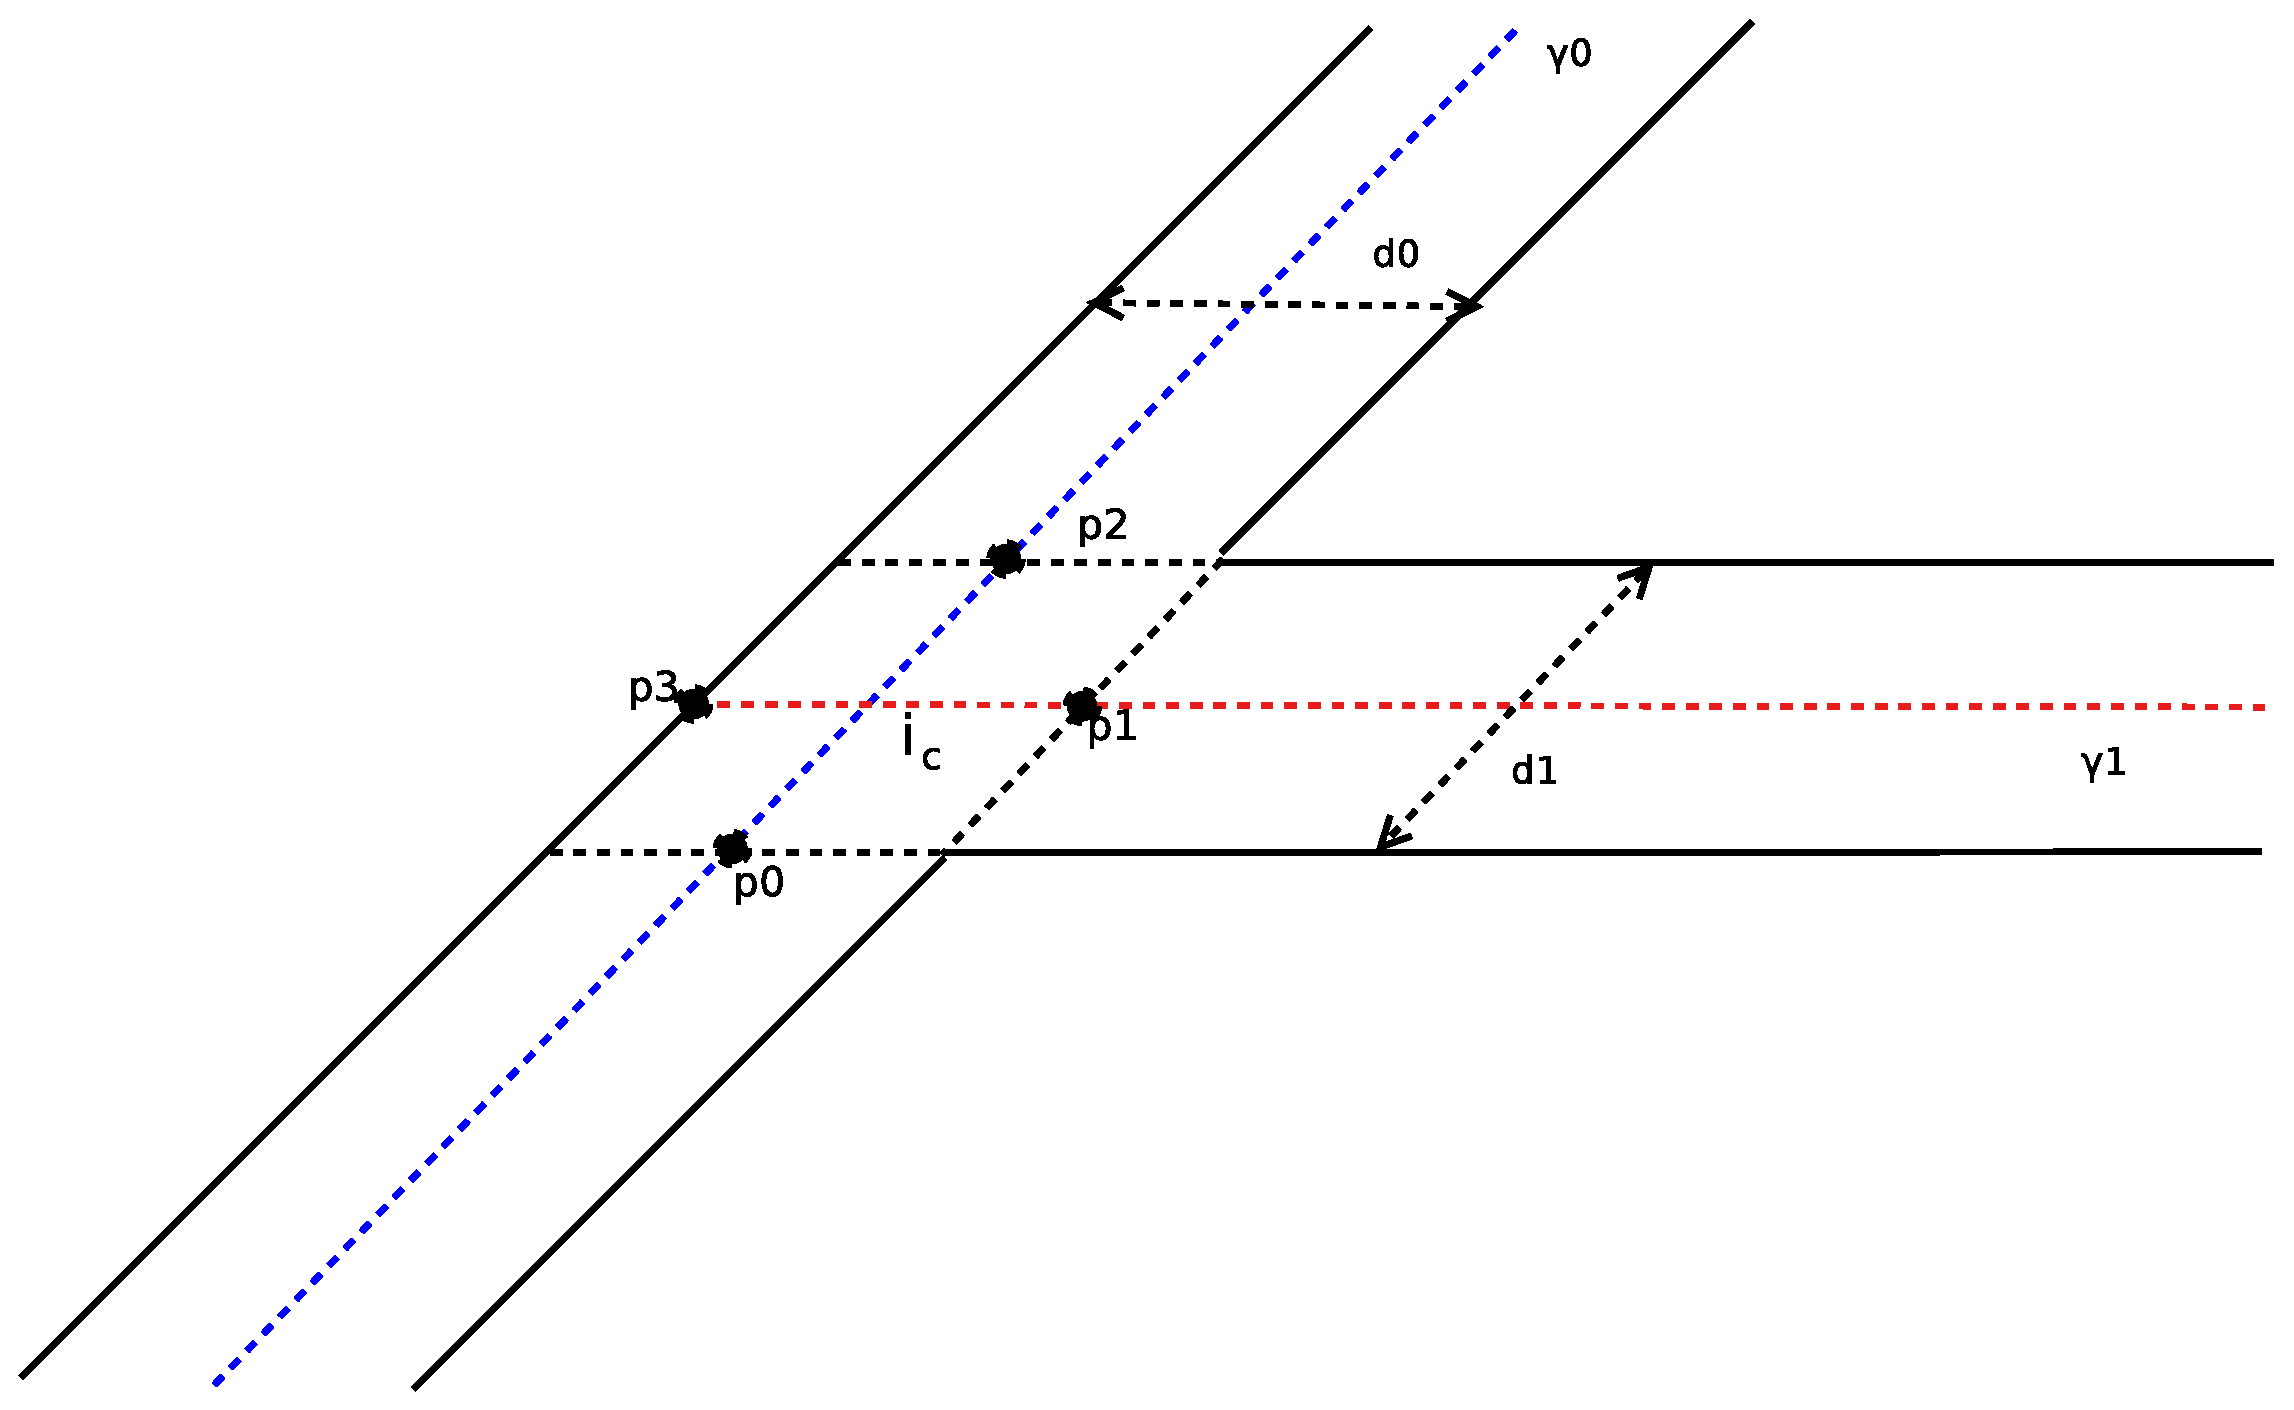
\includegraphics[width=0.8\textwidth]{img/cap6/y.eps}
\caption{Struttura di un'intersezione di tipo \textit{Bifurcation} tra due fratture.}\label{Y}
\end{center}
\end{figure}

A differenza di quanto visto fino ad ora, qui la regione d'intersezione non è più un triangolo, ma un parallelogramma. Si può generalizzare l'approssimazione fatta in \cite{Paper} con gli operatori mimetici, essendo generici e non legati al tipo di cella di integrazione su cui si lavora. \\
\noindent Il punto di intersezione $i_c$ rappresenta un punto generico per la frattura $\gamma_0$ in figura \ref{Y}, mentre per la frattura $\gamma_1$ rappresenta il primo o l'ultimo nodo. Questo punto non è detto che coincida con un nodo della mesh di $\gamma_0$ , in generale non sappiamo dove cadrà, per questo, per poter imporre le condizioni d'interfaccia in modo corretto, abbiamo introdotto per questa frattura dei gradi di libertà estesi: due per la velocità e uno per la pressione. È così possibile ottenere una miglior approssimazione del valore di velocità e pressione prima e dopo il punto di intersezione nell'elemento della mesh tagliato. \\
Esteso il codice di partenza per la costruzione del quadrilatero di intersezione, le condizioni d'interfaccia che vanno imposte hanno la stessa forma del caso delle tre fratture:

\begin{center}			
	$\left \{
		\begin{array}{l}	
	 		\textbf{u} - p_{I}T\textbf{1}_{3}+T \boldsymbol{\Pi}=0  \\ \\
     	 	\displaystyle \sum_{k=0}^3 u_{k} = p_{I} - \pi  \\
		\end{array}
	\right.$
\end{center} \label{condizioni d'interfaccia y }

\begin{figure}[htbp]
\begin{center}
\includegraphics[width=1.2\textwidth]{img/cap6/dipendenze.pdf}
\caption{Struttura globale del codice per il calcolo generico della matrice di trasmissibilità}\label{dipendenze}
\end{center}
\end{figure}


\noindent In questo caso cambiano però le dimensioni. La matrice di trasmissibilità $T$ è ora una matrice di $\mathbb{R}^{4 \times 4}$, come diretta conseguenza della natura delle matrici $C$ e $N$. Ora infatti l'area d'intersezione è delimitata da quattro lati. Anche lo scalare $\pi$ e il vettore $\boldsymbol{\Pi}$ cambiano, e diventano:
$$\boldsymbol{\Pi} = \left[ \begin{matrix}
 			p_0\\ 
 			p_1\\
 			p_2 \\ 
		 	p_3 \\
 			\end{matrix}\right] 
$$ 
 e
$$ \pi = \frac{p_0 + p_1 + p_2 + p_3 }{4} $$

Per poter imporre le condizioni d'interfaccia, per la frattura tagliata, è necessario usare il valore della pressione e della velocità a ridosso dell'intersezione, ma questi valori sono incogniti. 
Usiamo il grado classico di pressione e il grado esteso per indicare il valore di pressione prima e dopo il punto $i_c$, indicati con $p_0$ e $p_2$ in figura \ref{Y}.  L'incognita $p_1$ rappresenta il primo o l'ultimo grado di libertà della frattura $\gamma_1$, mentre con $p_3$ indichiamo un nodo fittizio, in cui imponiamo condizione di flusso nullo.

\noindent Per quanto riguarda la velocità invece, prima dell'intersezione la poniamo pari alla media tra il valore nel grado di libertà classico prima e il valore nel grado esteso dopo il punto $i_c$. Lo stesso facciamo per il valore di velocità dopo l'intersezione, come indicato in figura \ref{xfem}. \\

\newpage
\begin{figure}[htbp]
\begin{center}
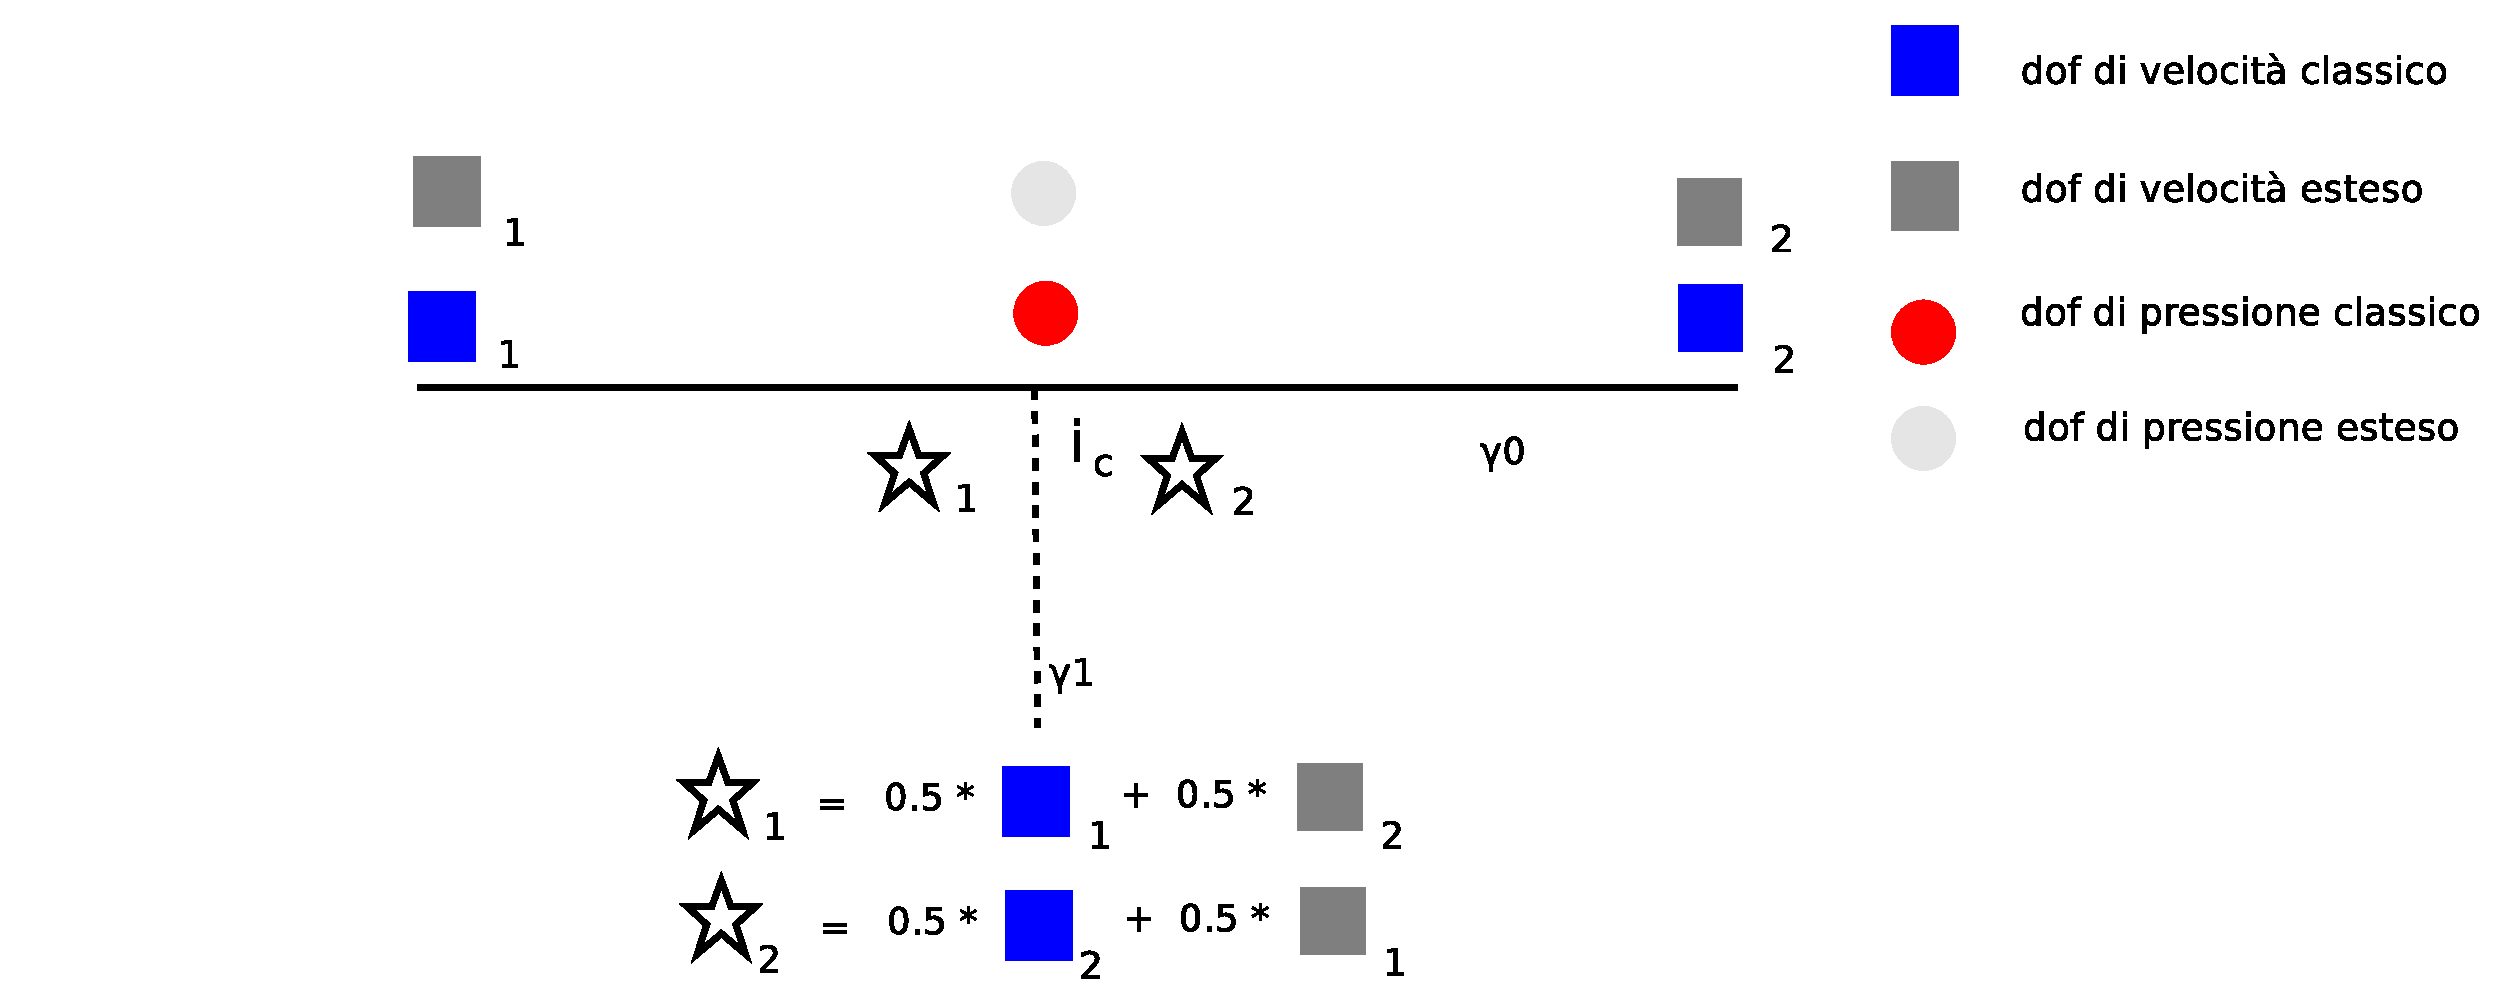
\includegraphics[width=1\textwidth]{img/cap6/xfem.eps}
\caption{Introduzione dei gradi di libertà estesi per la frattura tagliata.}\label{xfem}
\end{center}
\end{figure}

\subsection{Risultati numerici}
Ripetiamo l'analisi precedente per il caso particolare di biforcazione. Confronto valori della pressione nel DOF di intersezione per il modello 2D:\\
\begin{figure}[h!]
\centering
\includegraphics[scale=.45]{img/cap6/CP.eps}
\caption{Risultati \texttt{FreeFem++} biforcazione particolare risultati paraview }\label{CPParaview}
\end{figure}

\begin{center}
\begin{tabular}{|c|c|c|c|c|c|}
\hline
  & & \textbf{\texttt{Code}} & \multicolumn{3}{|c|}{\textbf{\texttt{FreeFem++}}} \\
\hline
\multicolumn{1}{|c|}{Frattura} & DOF & - &
\multicolumn{1}{|c|}{1E-01} & 1E-02 & 1E-03 \\
\hline
\multirow{2}{*}{0} & Base & 0.0480334 & 0.686998 & 0.303247 & 0.00685515\\
\cline{2-6}
& Esteso & 0.00295565 & 0.737573 & 0.307976 & 0.00665541\\
\hline
 1 & Base & 0.0146871 & 0.637801 & 0.298043 & 0.00673082\\
\hline
\end{tabular}
\end{center}

\begin{center}
\begin{tabular}{|c|c|c|c|}
\hline
\multicolumn{4}{|c|}{Pressione media} \\
\hline
\textbf{\texttt{Code}} & \multicolumn{3}{|c|}{\textbf{\texttt{FreeFem++}}} \\
\hline
- & \multicolumn{1}{|c|}{1E-01} & 1E-02 & 1E-03 \\
\hline
0.02189205 & 0.679653 & 0.301661 & 0.00672457 \\
\hline
\end{tabular}
\end{center}

\begin{figure}[h!]
\centering
\includegraphics[scale=.07]{img/cap6/BifuY.eps}
\caption{Risultati \texttt{FreeFem++} biforcazione con due fratture - spessore ordine 1E-02 }\label{Biforcazione2Frat1E-02}
\end{figure}

\begin{center}
\begin{tabular}{|c|c|c|}
\hline
  \multicolumn{3}{|c|}{\textbf{\texttt{Errore}}} \\ 
\hline
\multicolumn{1}{|c|}{1E-01} & 1E-02 & 1E-03 \\
\hline
0.65776095 & 0.27976895 & 0.01516748 \\
\hline
\end{tabular}
\end{center}

\subsection{Conclusioni}
Dal confronto dei risultati ottenuti con il nostro codice e con i codici \texttt{FreeFem++} possiamo concludere che effettivamente il modello ridotto da noi usato rappresenta una buona approssimazione del fenomeno. L'approssimazione è tanto migliore quanto più le fratture hanno uno spessore piccolo, come avevamo già previsto. Infatti più sono grandi e più informazioni trascuriamo usando un modello 1d. \\
\noindent Si potrebbe generalizzare ulteriormente il codice, usando sempre gli operatori mimetici, al caso in cui vi sia un numero generico di fratture che si intersecano in un punto. 


%\include{bibliografia.bib}

\bibliographystyle{plain}
\bibliography{bibliografia}

\include{appendice}

\end{document}




\begin{tikzpicture}[remember picture,overlay]
\node [opacity=0.2,scale=0.2] at (current page.center) {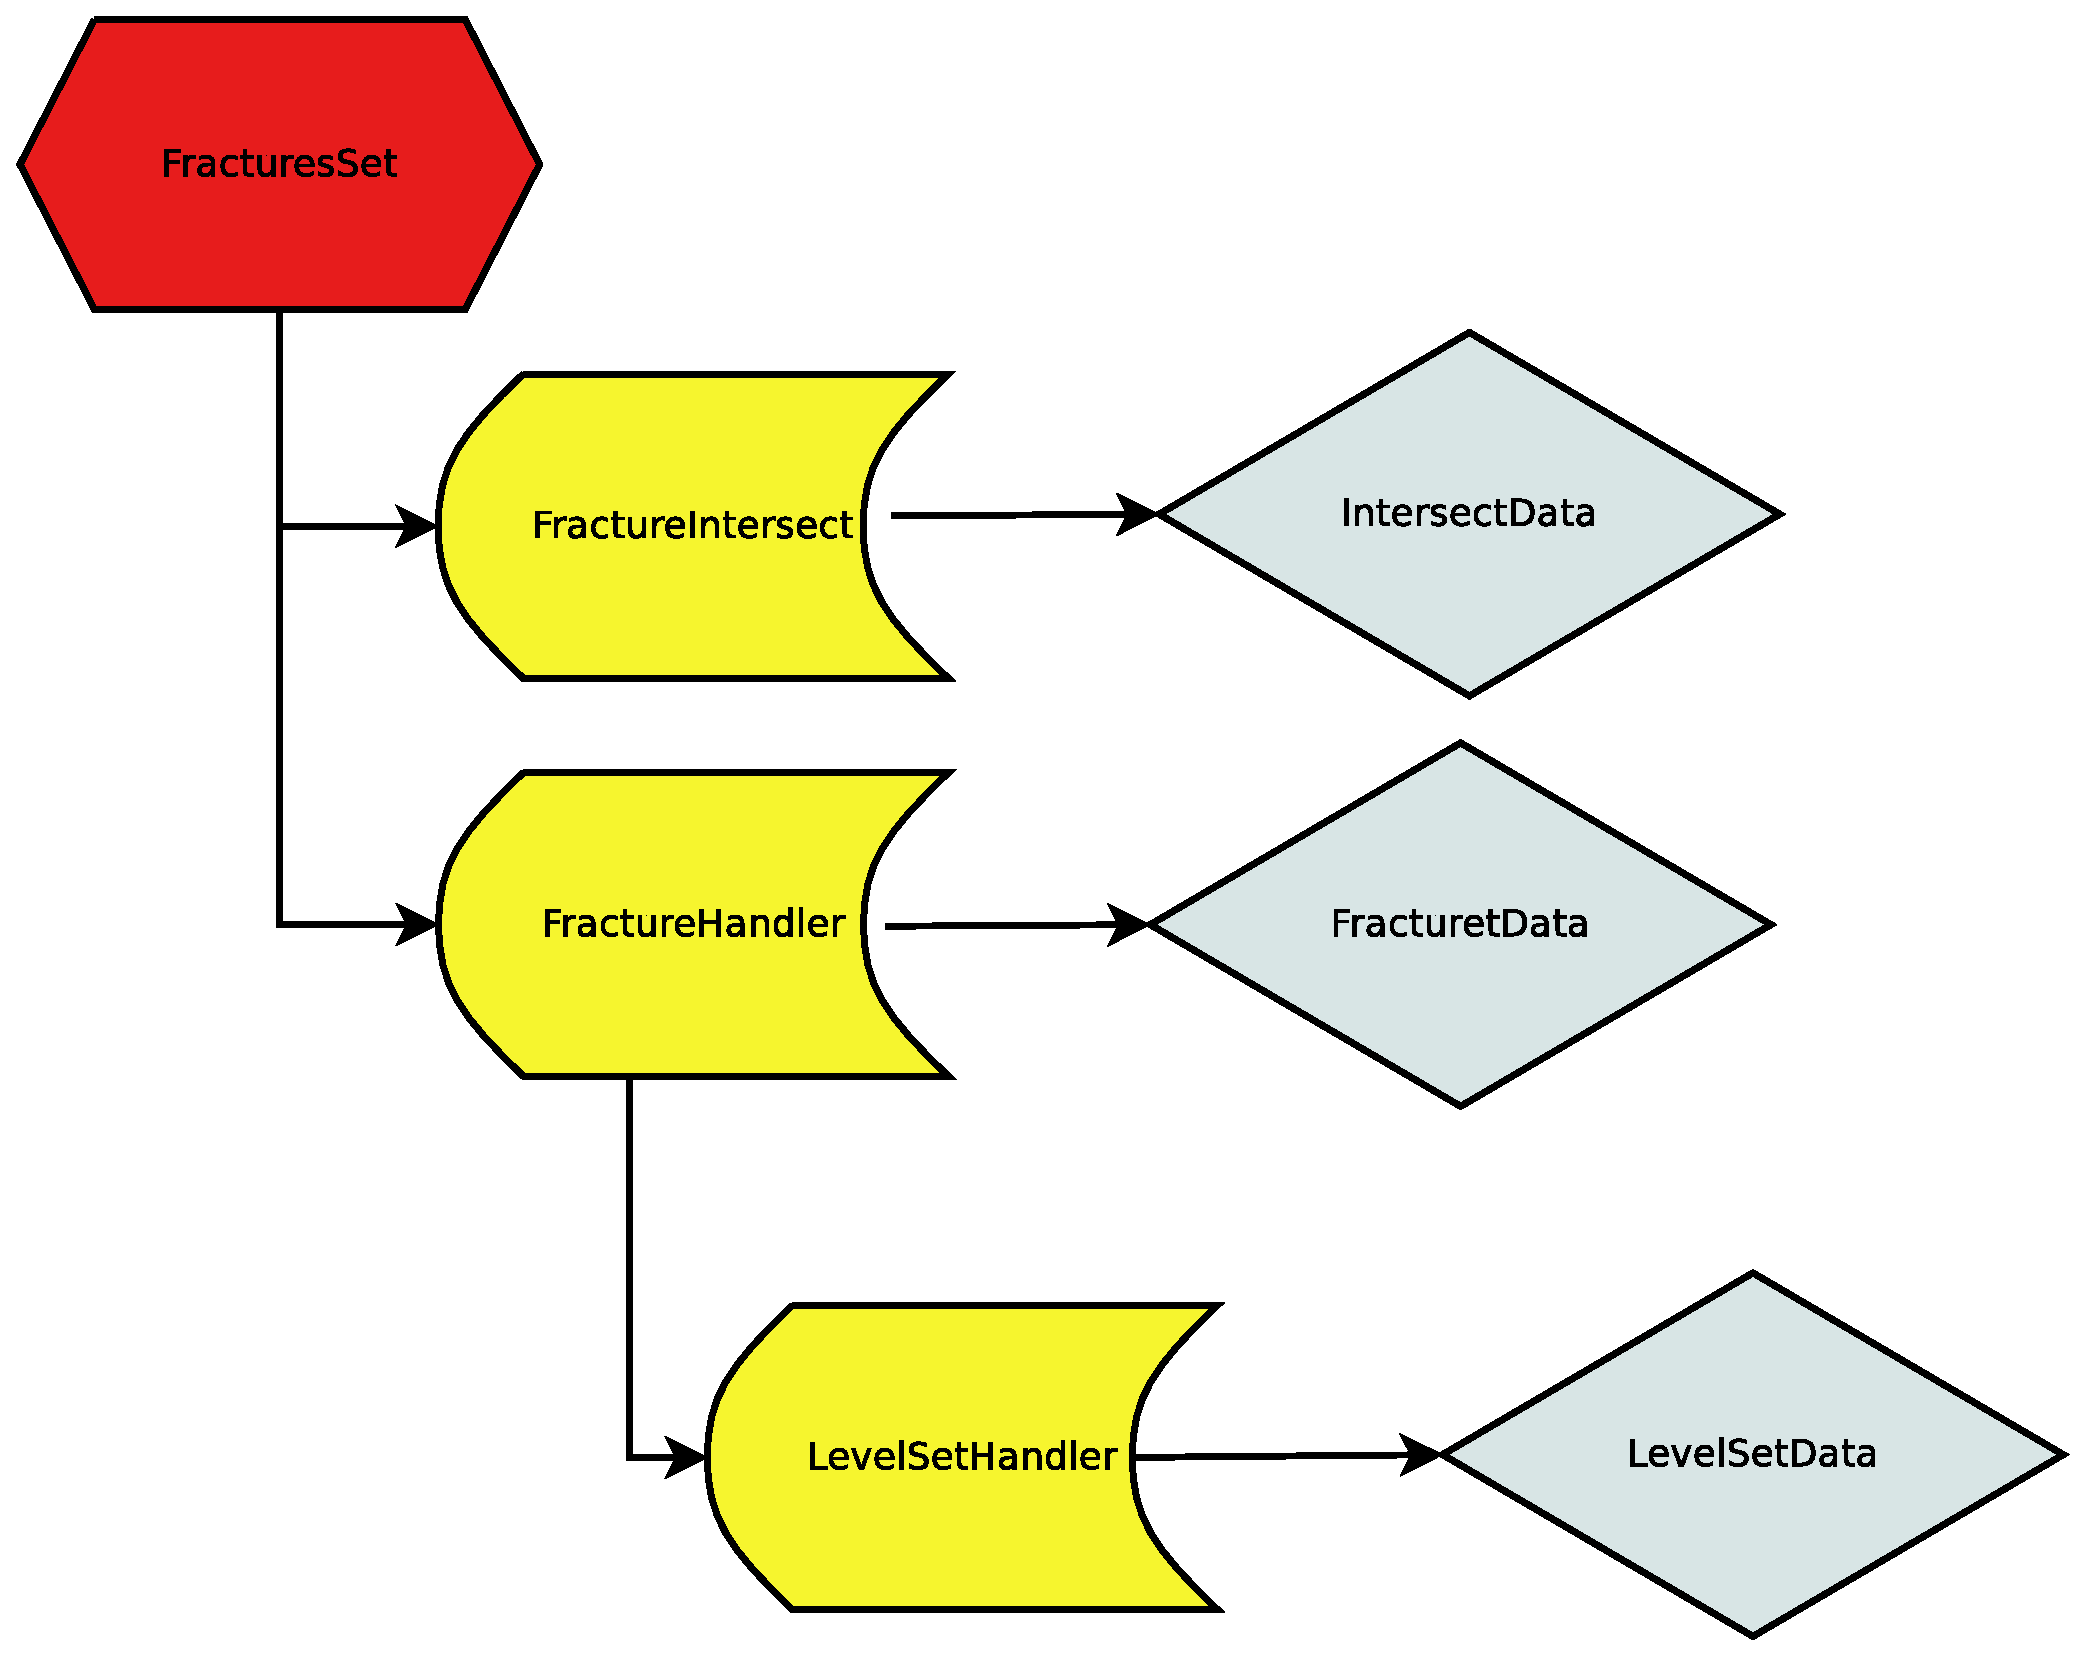
\includegraphics{img/fratture.eps}};
\end{tikzpicture}
